\documentclass[bachelor, och, nir]{SCWorks}
% параметр - тип обучения - одно из значений:
%    spec     - специальность
%    bachelor - бакалавриат (по умолчанию)
%    master   - магистратура
% параметр - форма обучения - одно из значений:
%    och   - очное (по умолчанию)
%    zaoch - заочное
% параметр - тип работы - одно из значений:
%    referat    - реферат
%    coursework - курсовая работа (по умолчанию)
%    diploma    - дипломная работа
%    pract      - отчет по практике
% параметр - включение шрифта
%    times    - включение шрифта Times New Roman (если установлен)
%               по умолчанию выключен
\usepackage{subfigure}
\usepackage{tikz,pgfplots}
\pgfplotsset{compat=1.5}
\usepackage{float}

%\usepackage{titlesec}
\setcounter{secnumdepth}{4}
%\titleformat{\paragraph}
%{\normalfont\normalsize}{\theparagraph}{1em}{}
%\titlespacing*{\paragraph}
%{35.5pt}{3.25ex plus 1ex minus .2ex}{1.5ex plus .2ex}

\titleformat{\paragraph}[block]
{\hspace{1.25cm}\normalfont}
{\theparagraph}{1ex}{}
\titlespacing{\paragraph}
{0cm}{2ex plus 1ex minus .2ex}{.4ex plus.2ex}

% --------------------------------------------------------------------------%
\usepackage[T2A]{fontenc}
\usepackage[utf8]{inputenc}
\usepackage{graphicx}
\graphicspath{ {./img/} }
\usepackage{tempora}

\usepackage[sort,compress]{cite}
\usepackage{amsmath}
\usepackage{amssymb}
\usepackage{amsthm}
\usepackage{fancyvrb}
\usepackage{listings}
\usepackage{listingsutf8}
\usepackage{longtable}
\usepackage{array}
\usepackage[english,russian]{babel}

\usepackage{url}
\usepackage[colorlinks=true, linkcolor=black]{hyperref}

\usepackage{underscore}
\usepackage{setspace}
\usepackage{indentfirst} 
\usepackage{mathtools}
\usepackage{amsfonts}
\usepackage{enumitem}
\usepackage{tikz}
\usepackage{textgreek}
\usepackage{diagbox}
\usepackage{caption}
\usepackage{float}
\usepackage{placeins}


% \usepackage{slashbox}
% \usepackage[justification=centering]{caption}
\usepackage[font=small,labelfont=bf,justification=centering]{caption}

\usepackage{minted}
\setminted[python3]{style=bw, linenos, breaklines=true, fontsize=\footnotesize}
\setminted[py]{fontsize=\small, breaklines=true, style=bw, linenos}

\newcommand{\eqdef}{\stackrel {\rm def}{=}}
\newcommand{\specialcell}[2][c]{%
\begin{tabular}[#1]{@{}c@{}}#2\end{tabular}}

\renewcommand\theFancyVerbLine{\small\arabic{FancyVerbLine}}

\newtheorem{lem}{Лемма}

\begin{document}

% Кафедра (в родительном падеже)
\chair{теоретических основ компьютерной безопасности и криптографии}

% Тема работы
\title{Слабое геодезическое число и число несократимости}

% Курс
\course{5}

% Группа
\group{531}

% Факультет (в родительном падеже) (по умолчанию "факультета КНиИТ")
\department{факультета КНиИТ}

% Специальность/направление код - наименование
%\napravlenie{09.03.04 "--- Программная инженерия}
%\napravlenie{010500 "--- Математическое обеспечение и администрирование информационных систем}
%\napravlenie{230100 "--- Информатика и вычислительная техника}
%\napravlenie{231000 "--- Программная инженерия}
\napravlenie{10.05.01 "--- Компьютерная безопасность}

% Для студентки. Для работы студента следующая команда не нужна.
\studenttitle{cтудентки}

% Фамилия, имя, отчество в родительном падеже
\author{Ивановой Ксении Владиславовны}

% % Заведующий кафедрой
% \chtitle{д. ф.-м. н., доцент} % степень, звание
% \chname{М.~Б.~Абросимов}

%Научный руководитель (для реферата преподаватель проверяющий работу)
\satitle{д. ф.-м. н., профессор} %должность, степень, звание
\saname{М.~Б.~Абросимов}

% Руководитель практики от организации (только для практики,
% для остальных типов работ не используется)
% \patitle{к.ф.-м.н.}
% \paname{С.~В.~Миронов}

% Семестр (только для практики, для остальных
% типов работ не используется)
%\term{8}

% Наименование практики (только для практики, для остальных
% типов работ не используется)
%\practtype{преддипломная}

% Продолжительность практики (количество недель) (только для практики,
% для остальных типов работ не используется)
%\duration{4}

% Даты начала и окончания практики (только для практики, для остальных
% типов работ не используется)
%\practStart{30.04.2019}
%\practFinish{27.05.2019}

% Год выполнения отчета
\date{2025}

\maketitle

% Включение нумерации рисунков, формул и таблиц по разделам
% (по умолчанию - нумерация сквозная)
% (допускается оба вида нумерации)
% \secNumbering

%-------------------------------------------------------------------------------------------

% \begin{minted}[fontsize=\small]{MySQL}
% \end{minted}

% \begin{figure}[H]
%     \centering
%     \includegraphics[width=0.999\textwidth]{img/}
%     \caption{}
%     \label{easy_hack}
% \end{figure}

\tableofcontents

\intro
В теории графов часто изучают числовые инварианты, чтобы лучше понять устройство графов и применять знания в решении сложных задач. Предлагаю остановиться на рассмотрении слабого геодезического числа и числа нескоратимости графа.

Обычно эти инварианты рассматривают отдельно и их связь почти не изучалась. Исследование того, как они связаны друг с другом, может дать новые интересные результаты о структуре графов. В этой работе мы проанализируем данные инварианты и их связь для всех графов до 11 вершин, попробуем выявить закономерности и составить галерею особенных графов.

\section{Теоретическая часть}

Расстоянием $d(u, v)$ между вершинами $u$ и $v$называется длина
кратчайшего пути между вершинами $u$ и $v$. Очевидно, что этот путь будет
цепью. Любой путь между вершинами $u$ и $v$ длины $d(u, v)$ называется 
геодезическим. 

\textbf{Геодезический граф} "---граф, в котором для любых двух вершин существует единственная
соединяющая их геодезическая цепь.

Все деревья являются геодезическими графами, так как любые
две вершины дерева соединены единственной цепью. Также геодезическими
графами являются полные графы и циклы нечётной длины. 

\textbf{Геодезическое множество} графа $G$ "--- множество его
вершин $S$ такое, что каждая вершина графа $G$ принадлежит какой-либо
геодезической, соединяющей пару вершин из $S$. 

\textbf{Минимальным} геодезическое множество называется, если никакое его 
собственное подмножество не является геодезическим множеством. 

\textbf{Геодезическое число} $g(G)$ графа $G$ "--- минимальная мощность 
его геодезического множества, а сами такие множества называются наименьшими 
геодезическими множествами. В некоторых работах вместо термина «геодезическое число» используется
термин <<число геодоминирования>>.

\textbf{Слабое геодезическое (геодоминирующее) множество} графа $G$ "---
множество его вершин $S$ такое, что каждая вершина графа $G$
слабо геодоминируется некоторой парой вершин из $S$. 

\textbf{Слабое геодезическое число} $wg(G)$ графа $G$ "---  минимальная мощность его слабого геодезического множества, а сами такие множества называются
наименьшими слабыми геодезическими множествами. Очевидно, что
$wg(G) \ge g(G)$, для полного графа $K_n: wg(K_n) = g(K_n) = n$    \cite{rad2008strong}, \cite{rad2008weak}.

 \textbf{Доминирующее множество} "--- это такое подмножество вершин $D \subseteq V$, 
 что любая вершина не из $D$ смежна хотя бы одной вершине из $D$. Говорят, 
 что вершины $v$ и $u$ доминируют друг друга, если в графе есть ребро $\{v, u\}$ или $v = u$[1].


\textbf{Несократимое множество} $D$ для графа $G$ "--- множество вершин, где для каждой
 вершины $v \in D$ выполняется условие $N[v] - N[S - \{v\}] \neq \varnothing$. 
 Другими словами, для любой вершины $v \in D$ или среди вершин графа не из $D$
 существует вершина, которая доминируется вершиной $v$ и не доминируется никакой 
 другой вершиной из $D$, или в $S$ нет вершин, смежных с $v$. Каждое минимальное 
 доминирующее множество является несократимым.

\textbf{Число несократимости} $ir(G)$ для графа $G$ "--- минимальная
мощность его максимального несократимого множества \cite{cockayne1978}.


\section{Алгоритмы} 
\subsection{Нахождение слабого геодезического числа}

Для нахождения вычисления слабого геодезического числа графа $wg(G)$ нужно найти такое минимальное множество вершин $S$, чтобы все вершины графа лежали на кратчайших путях между некоторыми парами вершин из множества $S$.

Для начала пронумеруем все вершины графа, и с помощью BFS вычислим кратчайшие расстояния от текущей до всех остальных. Так мы узнаем, какие вершины лежат на кратчайших путях между другими вершинами.

Для каждой пары вершин $(i, j)$ рассмотрим и сохраним множество всех таких вершин $k$, что $dist[i][k] + dist[k][j] = dist[i][j]$ (т.е. лежат на кратчайшем пути). 

Далее будем перебирать все возможные подмножества вершин графа (начиная с подмножеств размером 2). Для каждого будем вычислять объединение всех вершин, лежащих на кратчайших путях между его элементами. Если объединение покрывает все вершины графа, то размер этого множества будет являться выходом алгоритма. Если ни одно из меньших подмножеств не покрывает граф полностью, то выходом алгоритма будет количество вершин.
\vspace{1em}

\textbf{Алгоритм вычисления слабого геодезического числа графа}

\textit{Входные данные:} связный граф $G = (V, E)$.

\textit{Выходные данные:} слабое геодезическое число $wg(G)$ .

\underline{Шаг 1}. Пусть $n = |V|$. Если $n = 0$, вернуть $wg(G) = 0$.

\underline{Шаг 2}. Пронумеруем вершины $v_i \in V$, где $i \in \{0, \dots, n-1\}$.

\underline{Шаг 3}. Вычислим матрицу кратчайших расстояний $dist[i][j]$ между всеми 
  парами вершин графа $G$. Для каждой вершины $u \in V$ инициализируем $dist[u][u] = 0$, запускаем BFS из $u$, далее обновляем расстояния до остальных вершин.
  
\underline{Шаг 4}. Для каждой пары $(i,j)$, где $i < j$, посчитаем расстояние $d_{ij} = dist[i][j]$. Множество $P_{ij}$ всех вершин $k$ таких, что $dist[i][k] + dist[k][j] = d_{ij}$, закодируем битовой маской.
  
\underline{Шаг 5}. Зададим битовую маску $full = (1 \ll n) - 1$, соответствующую покрытию всех вершин графа.

\underline{Шаг 6}. Для каждого  $S_i \subseteq V$, где $ i \in \{2, \dots, n\}$:
 вычислим объединение всех <<геодезических областей>> пар $(u,v) \subseteq S_i$. Если объединение покрывает все вершины (битовая маска равна $full$), возвращаем $wg(G) = |S_i|$, иначе возвращаем $wg(G) = n$.

\subsection{Нахождение числа несократимости}

Чтобы найти число несократимости $ir(G)$, нужно исследовать все возможные подмножества вершин и вычислить наименьший размер такого максимального $S$, в котором ни одна вершина не является соседом с другой вершинами из $S$. 

Начнем с проверки, является ли множество пустым — в этом случае число несократимости графа будет равно нулю, иначе будем перебирать все возможные подмножества множества вершин $V$ и каждое подмножество будем проверять на несократимость. Множество считается несократимым, если для каждой его вершины $v$ существует хотя бы одна вершина $u$ в том же подмножестве, такая что $u \neq v$ и $u$ не смежна с $v$. Если вершины такое множество пусто, подмножество не будет являться несократимым.

Все выявленные несократимые подмножества будем проверять на максимальность. Для этого к каждому множеству будем поочерёдно добавлять все вершины, которые не входят в него, а далее проверять остаётся ли оно все еще несократимым. Если остается, тогда исходное множество является максимальным.

Среди всех найденных максимальных несократимых множеств выбираем то, которое имеет наименьший размер. Это и будет числом несократимости графа. Если ни одно множество не удовлетворяет условиям несократимости и максимальности, тогда $ir(G) = 1$.
\vspace{1em}

\textbf{Алгоритм вычисления числа несократимости графа}

\textit{Входные данные:} $G = (V, E)$.

\textit{Выходные данные:} число несократимости $ir(G)$.

\underline{Шаг 1}. Сначала проверим $V \neq \emptyset$, иначе вернем $ir(G) = 0$.

\underline{Шаг 2}. Определим $min\_size \leftarrow \infty$.

\underline{Шаг 3}. Для $S_i \subseteq V$, где $i \in \{0, \dots, n\}$, рассмотрим вершины $v_k \in S_i$, где $k \subseteq |S_i|$, и вычислим <<множество несоседей>> $pn(v_k, S_i)$ для каждой. Если для $v_k$ множество $pn(v_k, S_i) = \emptyset$, то $S_i$ не несократимое.

\underline{Шаг 4}. Из выборки несократимых $S_i$, выбираем максимальное таким образом:
\begin{enumerate}
    \item Для каждой вершины $w \in V \setminus S$ сформируем $S' = S \cup \{w\}$.
    \item Проверим несократимость  $S'$ (аналогично шагу 4).
    \item Если хотя бы одно такое $S'$ несократимо, то $S$ не максимально.
\end{enumerate}

\underline{Шаг 5}. Если $S$ несократимо и максимально, обновим значение минимального множества : $min\_size = \min(min\_size,\ |S|)$.

\underline{Шаг 6}. Если $min\_size = \infty$, возвращаем $ir(G) = 1$, иначе  $ir(G) = min\_size$.




\newpage
\section{Исследовательская часть}

\subsection{Экспериментальная среда}
Генерация всех графов в формате graph6  \cite{graph6} с заданным числом вершин была произведена с помощью консольной программы geng из пакета nauti \cite{nauty}, результаты генерации были записаны в файл, пример использования 
    \begin{verbatim}
    for i in$(seq 1 11)
    do 
      ./geng -c $i > res$i
    end
    \end{verbatim}


Для вычисления самих инвариантов была написана программа на языке Python.
Сначала происходит чтение графа из ранее сгенерированного файла. Обработка идёт параллельно т.к. используется модуль \texttt{multiprocessing}, что позволяет задействовать несколько процессоров сразу.

Каждый граф превращается в объект библиотеки NetworkX  \cite{networkx}. Затем для него последовательно вычисляются инварианты. Пока программа работает, она собирает статистику "--- сколько раз встретилась каждая пара значений этих двух инвариантов, полученные данные записываются в результирующую матрицу. В конце анализа для каждого файла программа выводит на экран и сохраняет в файл матрицу распределения значений, общее количество успешно обработанных графов, число ошибок и общее время работы.

Вычисления были произведены на персональном компьютере с данными характеристиками:
\begin{enumerate}
    \item Операционная система: Linux Ubuntu;
    \item Процессор: AMD Ryzen 5 2600 Six-Core Processor (12 ядер);
    \item Оперативная память: 32 ГБ;
    \item Тип системы: x64;
\end{enumerate}

\subsection{Результаты исследования}
На таблице можно увидеть, как соотносятся число вершин и число графов к времени работы программы.  

\begin{table}[H]
    \centering
    \label{tab:time}
    \begin{tabular}{|c|c|c|}
        \hline
        Число вершин & Число графов & Время работы \\ \hline
        1  & 1 & 0.01 с \\ \hline
        2  & 1 & 0.05 с \\ \hline
        3  & 2 & 0.3 с \\ \hline
        4  & 6 & 0.3 с \\ \hline
        5  & 21 & 0.3 с \\ \hline
        6  & 112 & 0.5 с \\ \hline
        7  & 853 & 0.7 с \\ \hline
        8  & 11117 & 2.23 с \\ \hline
        9  & 261080 & 1.2 мин \\ \hline
        10 & 11716571 & 2 ч \\ \hline
        11 & 1006700565 & 16 дней \\ \hline
    \end{tabular}
\end{table}
\begin{center}
  \small\textbf{Таблица 1} -- Время работы программы
\end{center}

\vspace{0.5em}

На следующих таблицах отражены полученные в ходе вычислений результаты
для графов до 11 вершин.


\begin{table}[H]
    \centering
    \begin{tabular}{|c|c|}
    \hline
    \backslashbox[60pt]{\small$wg(G)$}{\small$ir(G)$} & 1 \\ \hline
    2                                     & 1 \\ \hline
    \end{tabular}
    \begin{center}
    \small\textbf{Таблица 2} -- Количество 2-вершинных графов со значениями заданных инвариантов.
    \end{center}
\end{table}


\vspace{0.5em}

\begin{table}[H]
    \centering
    \begin{tabular}{|c|c|c|}
    \hline
    \backslashbox[60pt]{\small$wg(G)$}{\small$ir(G)$} & 2 & 3 \\ \hline
    1 & 1 & 0  \\ \hline
    2 & 0 & 1  \\ \hline
    \end{tabular}
    \begin{center}
    \small\textbf{Таблица 3} -- Количество 3-вершинных графов со значениями заданных инвариантов.
    \end{center}
\end{table}

\vspace{0.5em}

\begin{table}[H]
    \centering
    \begin{tabular}{|c|c|c|c|}
    \hline
    \backslashbox[60pt]{\small$wg(G)$}{\small$ir(G)$} & 2 & 3 & 4 \\ \hline
    1  & 1 & 2  & 0 \\ \hline
    2  & 2  & 0 & 0 \\ \hline
    3  & 0  & 0 & 1 \\ \hline
    \end{tabular}
    \begin{center}
    \small\textbf{Таблица 3} -- Количество 4-вершинных графов со значениями заданных инвариантов.
    \end{center}
\end{table}


\vspace{0.5em}

\begin{table}[H]
    \centering
    \begin{tabular}{|c|c|c|c|c|}
    \hline
    \backslashbox[60pt]{\small$wg(G)$}{\small$ir(G)$} & 2 & 3 & 4 & 5\\ \hline
    1 & 3 & 4 & 4 & 0 \\ \hline
    2 & 2 & 5 & 0 & 0 \\ \hline
    3 & 2 & 0 & 0 & 0 \\ \hline
    4 & 0 & 0 & 0 & 1 \\ \hline
    \end{tabular}
    \begin{center}
    \small\textbf{Таблица 4} -- Количество 5-вершинных графов со значениями заданных инвариантов.
    \end{center}
\end{table}
\vspace{0.5em}


\begin{table}[H]
    \centering
    \begin{tabular}{|c|c|c|c|c|c|}
    \hline
    \backslashbox[60pt]{\small$wg(G)$}{\small$ir(G)$} & 2 & 3 & 4 & 5 & 6\\ \hline
    1 & 9 & 26 & 15 & 6 & 0 \\ \hline
    2 & 14 & 17 & 8 & 0 & 0 \\ \hline
    3 & 3 & 10 & 0 & 0 & 0 \\ \hline
    4 & 3 & 0 & 0 & 0 & 0 \\ \hline
    5 & 0 & 0 & 0 & 0 & 1 \\ \hline
    \end{tabular}
    \begin{center}
    \small\textbf{Таблица 5} -- Количество 6-вершинных графов со значениями заданных инвариантов.
    \end{center}
\end{table}

\vspace{0.5em}


\begin{table}[H]
    \centering
    \begin{tabular}{|c|c|c|c|c|c|c|}   
    \hline
    \backslashbox[60pt]{\small$wg(G)$}{\small$ir(G)$} 
    & 2  & 3   & 4  & 5 & 6 & 7          \\ \hline
    1 & 39 & 171  & 126  & 39 & 10 & 0    \\ \hline
    2 & 69  & 173  & 76  & 14 & 0 & 0    \\ \hline
    3 & 11 & 84 & 16  & 0 & 0 & 0    \\ \hline
    4 & 7 & 14 & 0 & 0 & 0 & 0    \\ \hline
    5 & 3 & 0 & 0 & 0 & 0 & 0    \\ \hline
    6 & 0 & 0 & 0 & 0 & 0 & 1    \\ \hline
    \end{tabular}
    \begin{center}
    \small\textbf{Таблица 6} -- Количество 7-вершинных графов со значениями заданных инвариантов.
    \end{center}
\end{table}
\vspace{0.5em}


\begin{table}[H]
    \centering
    \begin{tabular}{|c|c|c|c|c|c|c|c|}
    \hline  \backslashbox[60pt]{\small$wg(G)$}{\small$ir(G)$}
     & 2   & 3  & 4  & 5 & 6 & 7 & 8 \\ \hline
    1 & 219    & 1601   & 1593   & 473   & 94  & 14 & 0   \\ \hline
    2 & 608    & 2363   & 1529   & 211   & 24  & 0 & 0    \\ \hline
    3 & 268  & 1150     & 560   & 26  & 0  & 0 & 0  \\ \hline
    4 & 39    & 255    & 51     & 0  & 0  & 0 & 0  \\ \hline
    5 & 13   & 21     & 0   & 0   & 0  & 0 & 0  \\ \hline
    6 & 4    & 0     & 0   & 0   & 0  & 0 & 0  \\ \hline
    7 & 0    & 0     & 0   & 0   & 0  & 0 & 1  \\ \hline
    \end{tabular}
\end{table}
\begin{center}
  \small\textbf{Таблица 7} -- Количество 8-вершинных графов со значениями заданных инвариантов.
\end{center}

\vspace{0.5em}

\begin{table}[H]
    \centering
    \begin{tabular}{|c|c|c|c|c|c|c|c|c|}
    \hline  \backslashbox[60pt]{\small$wg(G)$}{\small$ir(G)$}
      & 2    & 3  & 4 & 5  & 6 & 7  & 8 & 9           \\ \hline
    1   & 2055 & 21540 & 32384 & 9259 & 1554 & 201 & 21 & 0 \\ \hline
    2   & 7400 & 49476 & 48283 & 7406 & 574  & 37  & 0  & 0 \\\hline
    3   & 7347 & 31324 & 26424 & 1268 & 47   & 0   & 0  & 0 \\\hline
    4   & 332  & 9792  & 3257  & 48   & 0    & 0   & 0  & 0 \\\hline
    5   & 111  & 799   & 82    & 0    & 0    & 0   & 0  & 0 \\\hline
    6   & 21   & 33    & 0     & 0    & 0    & 0   & 0  & 0 \\\hline
    7   & 4    & 0     & 0     & 0    & 0    & 0   & 0  & 0 \\\hline
    8   & 0    & 0     & 0     & 0    & 0    & 0   & 0  & 1 \\\hline
    \end{tabular}
    \begin{center}
    \small\textbf{Таблица 8} -- Количество 9-вершинных графов со значениями заданных инвариантов.
    \end{center}
\end{table}
\vspace{0.5em}

\begin{table}[H]
    \centering
    \begin{tabular}{|c|c|c|c|c|c|c|c|c|c|c|}
    \hline  \backslashbox[60pt]{\small$wg(G)$}{\small$ir(G)$}
    & 2 & 3 & 4 & 5  & 6  & 7  & 8  & 9 & 10\\ \hline
    1   & 33819  & 475821  & 1084140 & 330706 & 43520 & 4584 & 410 & 29 & 0 \\   \hline 
    2   & 158786 & 1623761 & 2362193 & 453457 & 29823 & 1385 & 58  & 0 & 0 \\   \hline 
    3   & 267603 & 1477177 & 2012307 & 141949 & 3234  & 74   & 0   & 0  & 0\\   \hline 
    4   & 55005  & 529624  & 519695  & 4706   & 75    & 0    & 0   & 0 & 0 \\   \hline 
    5   & 2004   & 79799   & 17547   & 69     & 0     & 0    & 0   & 0 & 0 \\   \hline 
    6   & 345    & 2586    & 193     & 0      & 0     & 0    & 0   & 0  & 0\\   \hline 
    7   & 34     & 47      & 0       & 0      & 0     & 0    & 0   & 0  & 0\\   \hline 
    8   & 5      & 0       & 0       & 0      & 0     & 0    & 0   & 0  & 0\\   \hline 
    9   & 0      & 0       & 0       & 0      & 0     & 0    & 0   & 0  & 1\\   \hline
    \end{tabular}
    \begin{center}
    \small\textbf{Таблица 9} -- Количество 10-вершинных графов со значениями заданных инвариантов.
    \end{center}
\end{table}
\vspace{0.5em}

\begin{table}[H]
    \centering
    \begin{tabular}{|c|c|c|c|c|c|}
    \hline  \backslashbox[60pt]{\small$wg(G)$}{\small$ir(G)$}
     & 2 & 3 & 4 & 5 & 6  \\ \hline
     1 & 2\,905\,766 & 40\,883\,063 & 93\,150\,496 & 28\,414\,623 & 3\,739\,286 \\ \hline
    2 & 13\,643\,068 & 139\,515\,329 & 202\,962\,217 & 38\,961\,524 & 2\,562\,425 \\ \hline
    3 & 22\,992\,744 & 126\,920\,671 & 172\,899\,628 & 12\,196\,414 & 277\,869 \\ \hline
    4 & 4\,726\,090 & 45\,505\,876 & 44\,652\,765 & 404\,345 & 6\,444 \\ \hline
    5 & 172\,186 & 6\,856\,418 & 1\,507\,658 & 5\,929 & 56 \\ \hline
    6 & 29\,643 & 222\,192 & 16\,583 & 27 & 0 \\  \hline
    7 & 2\,921 & 4\,038 & 43 & 0 & 0 \\ \hline
    8 & 98 & 34 & 0 & 0 & 0 \\ \hline
    9 & 5 & 0 & 0 & 0 & 0 \\ \hline
    10 & 0 & 0 & 0 & 0 & 0 \\ \hline
    \end{tabular}
    \begin{center}
    \small\textbf{Таблица 10.1} -- Количество 11-вершинных графов со значениями заданных инвариантов.
    \end{center}
\end{table}
\vspace{0.5em}


\begin{table}[H]
    \centering
    \begin{tabular}{|c|c|c|c|c|c|}
    \hline  \backslashbox[60pt]{\small$wg(G)$}{\small$ir(G)$}
     & 7 & 8 & 9 & 10 & 11 \\ \hline
     1 & 393\,862 & 35\,228 & 976 & 46 & 0 \\
    2 & 119\,001 & 4\,983 & 82 & 0 & 0 \\
    3 & 6\,358 & 75 & 0 & 0 & 0 \\
    4 & 32 & 0 & 0 & 0 & 0 \\
    5 & 0 & 0 & 0 & 0 & 0 \\
    6 & 0 & 0 & 0 & 0 & 0 \\
    7 & 0 & 0 & 0 & 0 & 0 \\
    8 & 0 & 0 & 0 & 0 & 0 \\
    9 & 0 & 0 & 0 & 0 & 0 \\
    10 & 0 & 0 & 0 & 0 & 1 \\
    \hline

    \end{tabular}
    \begin{center}
    \small\textbf{Таблица 10.2} -- Количество 11-вершинных графов со значениями заданных инвариантов.
    \end{center}
\end{table}
\vspace{0.5em}


\newpage
\subsection{Построение гипотез}
% \subsubsection*{Построение гипотез}
\textbf{Общие наблюдения}
\begin{enumerate}
    \item С ростом числа вершин максимальные значения для слабого геодезичсекого числа сосредотачиваются в диапазоне от 1 до 3, числа несократимости "--- от 3 до 4;
    \item Значения вне центральных областей таблицы стремятся к нулю, что видно по резкому уменьшению числа графов с увеличением этих параметров;
    \item Матрица на побочной диагонали и под ней заполнена нулями, за исключением одного элемнта. Графы с большими значениями инфвариант уникальны, их структура близка к полным или сильно связанным графам.
\end{enumerate}

\vspace{0.5em}
\textbf{Гипотеза 1.} 

Для множества графов с $n$ вершинами, максимальными возможными значениями слабого геодезического числа и числа несократимости будут $wg(G) = n-1$ и $ir(G) = n$, причем такой граф будет только один. Визуально закономерность можно увидеть на рисунках \ref{fig:im1}, \ref{fig:im2} , \ref{fig:im3}.
\begin{figure}[ht!]  
    \centering 
    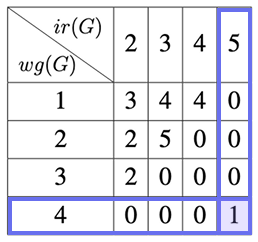
\includegraphics[width=0.3\textwidth]
{Group423.png}  
    \caption{Матрица отношений инвариантов для $n = 5$} 
    \label{fig:im1} 
\end{figure}

\begin{figure}[ht!]  
    \centering 
    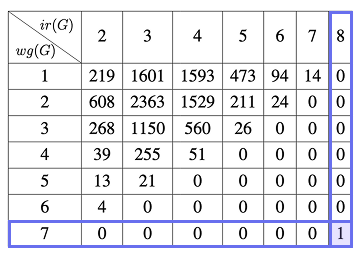
\includegraphics[width=0.5\textwidth]
{Group424.png}  
    \caption{Матрица отношений инвариантов для $n = 8$} 
    \label{fig:im2} 
\end{figure}

\begin{figure}[ht!]  
    \centering 
    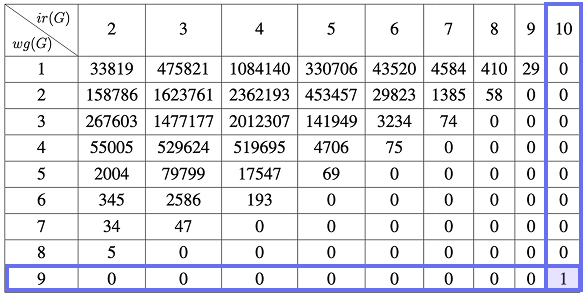
\includegraphics[width=0.8\textwidth]
{Group425.png}  
    \caption{Матрица отношений инвариантов для $n = 10$} 
    \label{fig:im3} 
\end{figure}

\textbf{Гипотеза 2.} 

Для множества графов с $n$ вершинами, не существует графа $G$ который будет обладать равными инвариантами: $ir(G) = wg(G) = K$, со значением $K >$ $\left\lfloor \displaystyle \frac{n}{2} \right\rfloor$. Визуально закономерность видна на рисунках \ref{fig:im4}, \ref{fig:im5} , \ref{fig:im6}.



\begin{figure}[ht!]  
    \centering 
    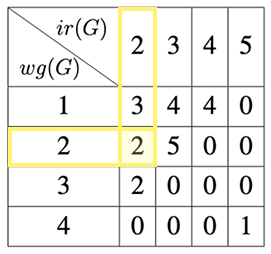
\includegraphics[width=0.3\textwidth]
{Group426.png}  
    \caption{Матрица отношений инвариантов для $n = 5$} 
    \label{fig:im4} 
\end{figure}


\begin{figure}[ht!]  
    \centering 
    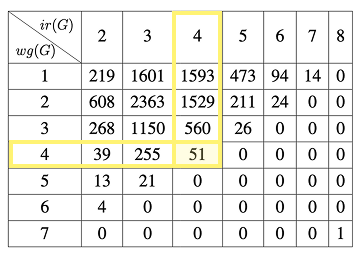
\includegraphics[width=0.5\textwidth]
    {Group427.png}  
    \caption{Матрица отношений инвариантов для $n = 8$} 
    \label{fig:im5} 
\end{figure}


\begin{figure} 
    \centering 
    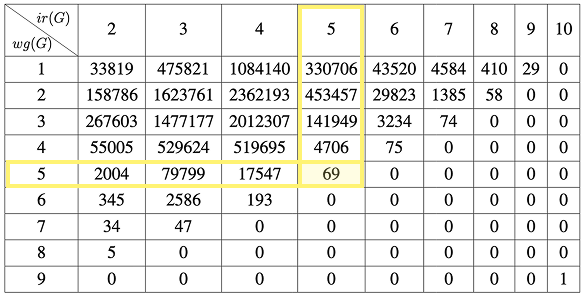
\includegraphics[width=0.8\textwidth]
{Group428.png}  
    \caption{Матрица отношений инвариантов для $n = 10$} 
    \label{fig:im6} 
\end{figure}

\newpage
\textbf{Гипотеза 3.}

Для множества графов с $n$ вершинами, будет существовать ровно $C =\left\lfloor \displaystyle \frac{n}{2} \right\rfloor$ графов со слабым геодезическим числом $wg(G) = n-2$ и числом несократимости $ir(G) = 2$. Визуально закономерность видна на рисунках
\ref{fig:im7}, \ref{fig:im8} , \ref{fig:im9}.



\begin{figure}[ht!]  
    \centering 
    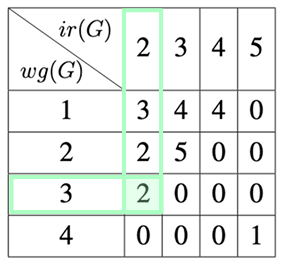
\includegraphics[width=0.3\textwidth]
{Group429.png}  
    \caption{Матрица отношений инвариантов для $n = 5$} 
    \label{fig:im7} 
\end{figure}
\FloatBarrier

\begin{figure}[ht!]  
    \centering 
    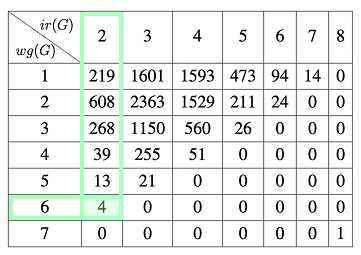
\includegraphics[width=0.5\textwidth]
    {Group430.png}  
    \caption{Матрица отношений инвариантов для $n = 8$} 
    \label{fig:im8} 
\end{figure}
\FloatBarrier


\begin{figure}[ht!]  
    \centering 
    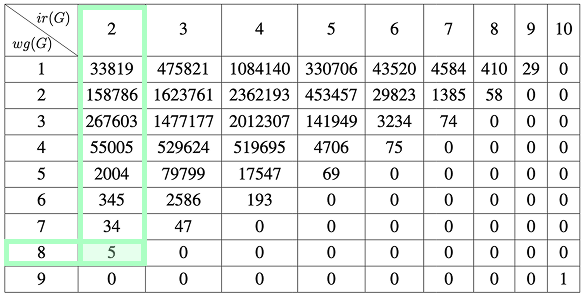
\includegraphics[width=0.8\textwidth]
{Group431.png}  
    \caption{Матрица отношений инвариантов для $n = 10$} 
    \label{fig:im9} 
\end{figure}



\section{Каталог графов}
На рисунках 10-19 представлены графы соответствующие гипотезе 1.

\begin{figure}[ht!]  
    \centering 
    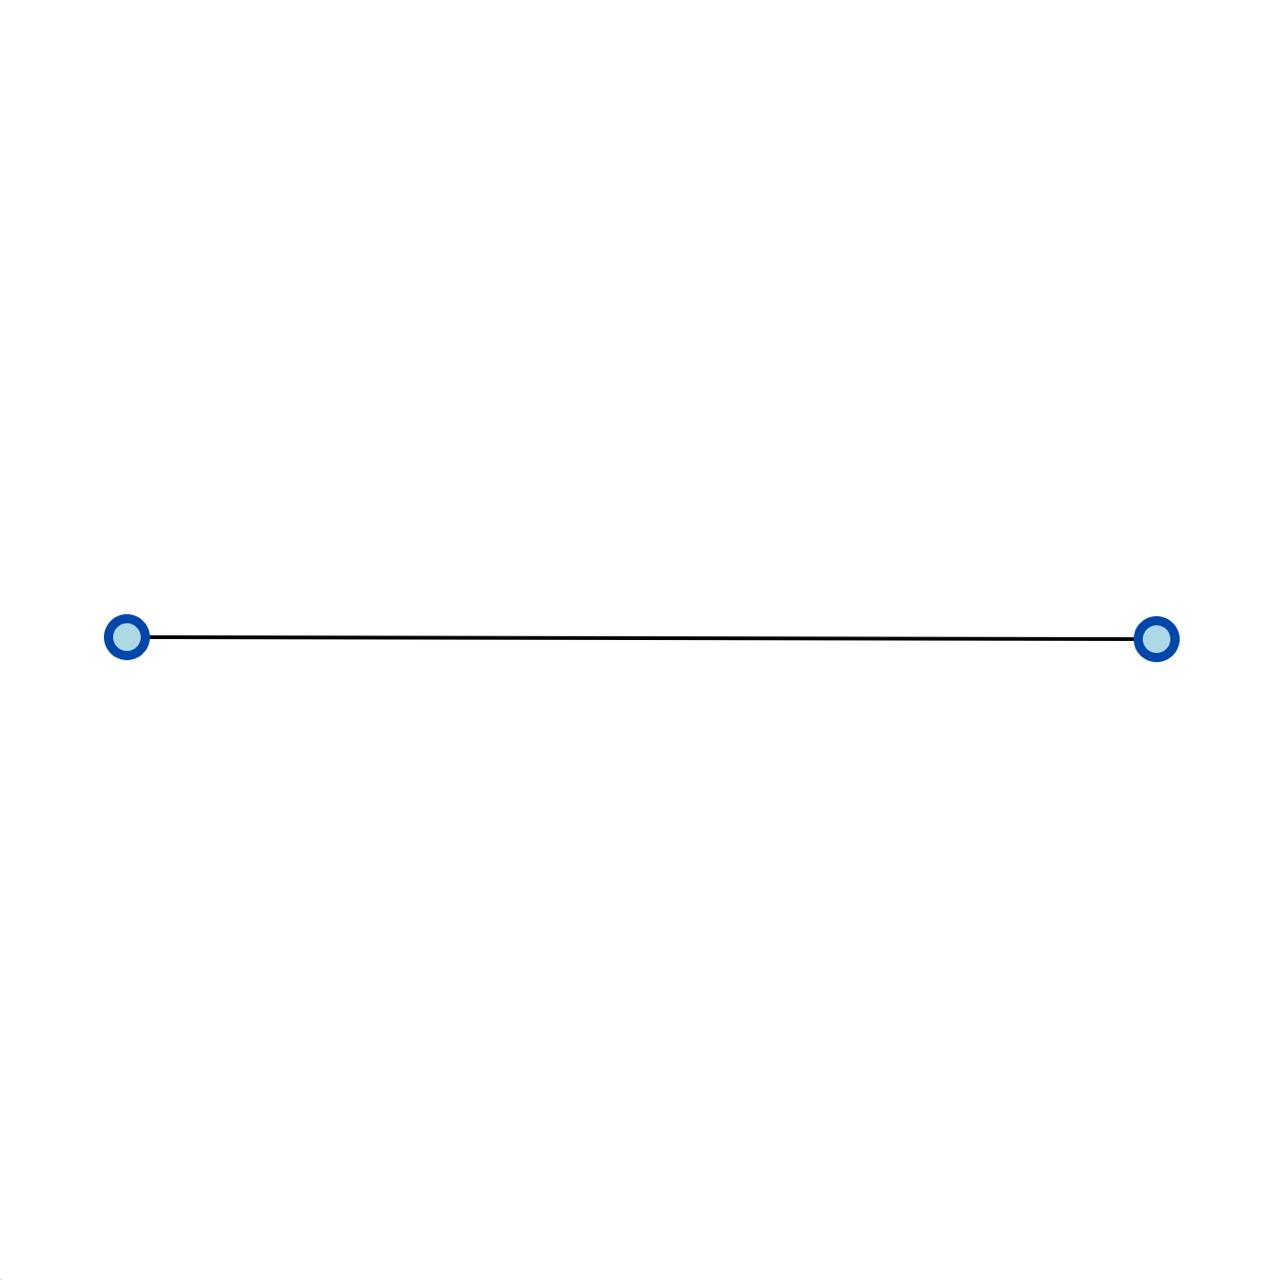
\includegraphics[width=0.5\textwidth]
{1.jpeg}  
    \caption{Граф $wg(G) = 2, ir(G) = 1$} 
    \label{fig:im2} 
\end{figure}


\begin{figure}[ht!]  
    \centering 
    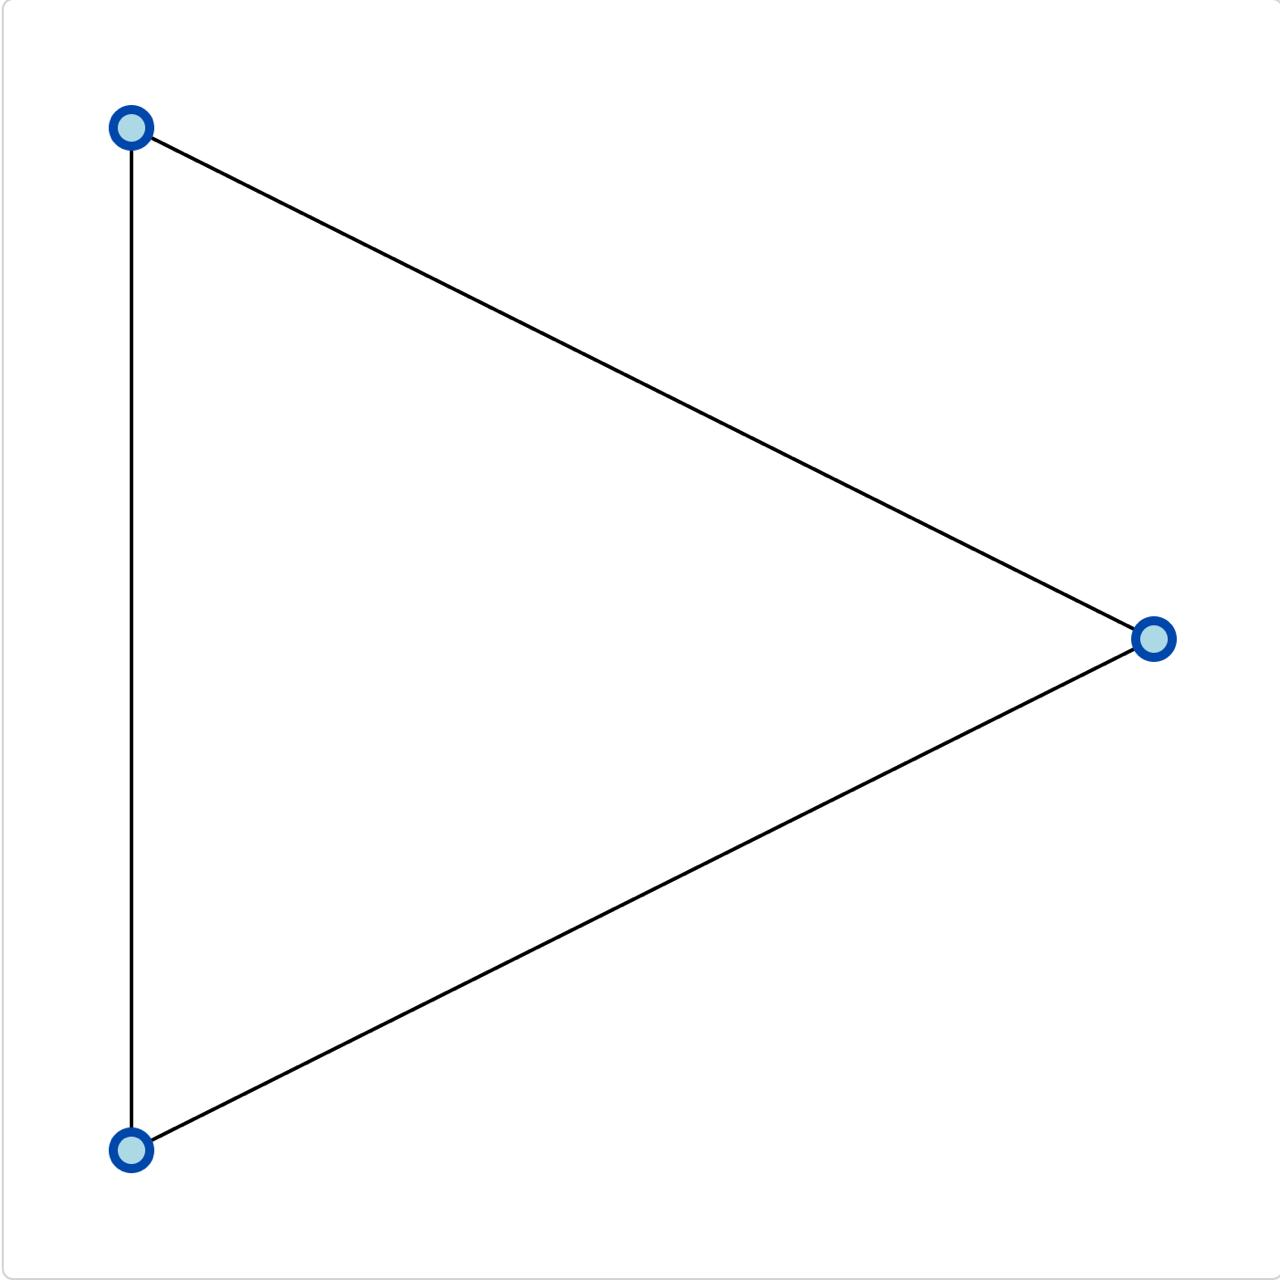
\includegraphics[width=0.5\textwidth]
{2.jpeg}  
    \caption{Граф $wg(G) = 2 , ir(G) = 3 $} 
    \label{fig:im2} 
\end{figure}

\begin{figure}[ht!]  
    \centering 
    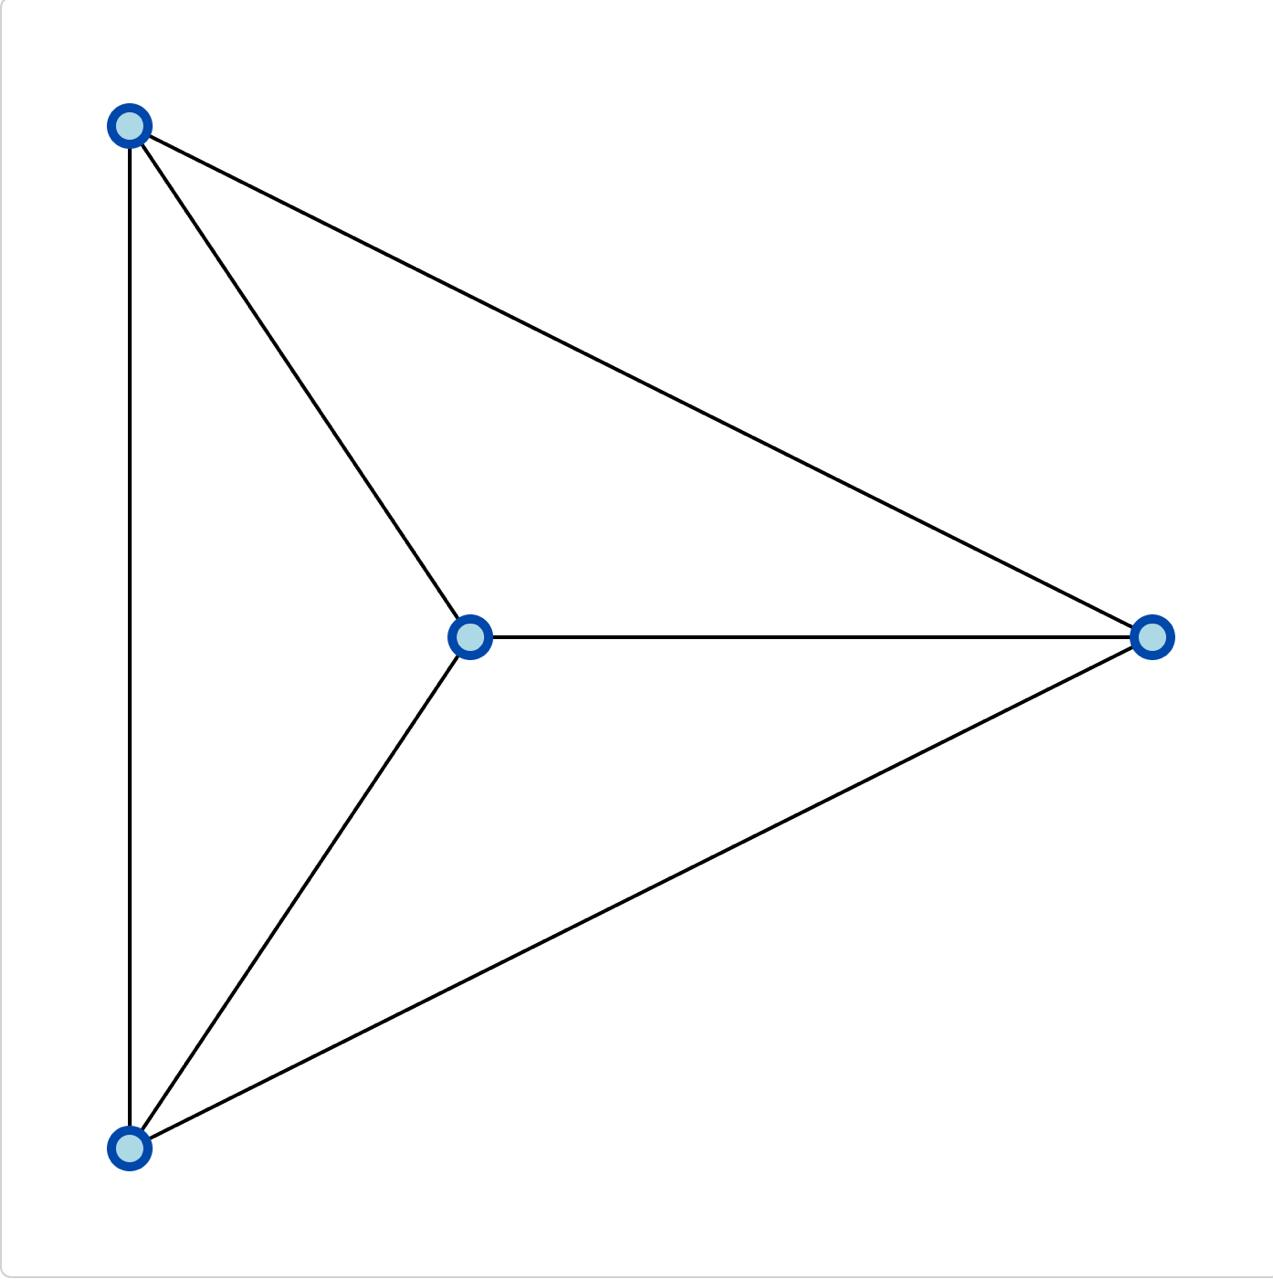
\includegraphics[width=0.5\textwidth]
{3.jpeg}  
    \caption{Граф $wg(G) = 3, ir(G) = 4$} 
    \label{fig:im2} 
\end{figure}

\begin{figure}[ht!]  
    \centering 
    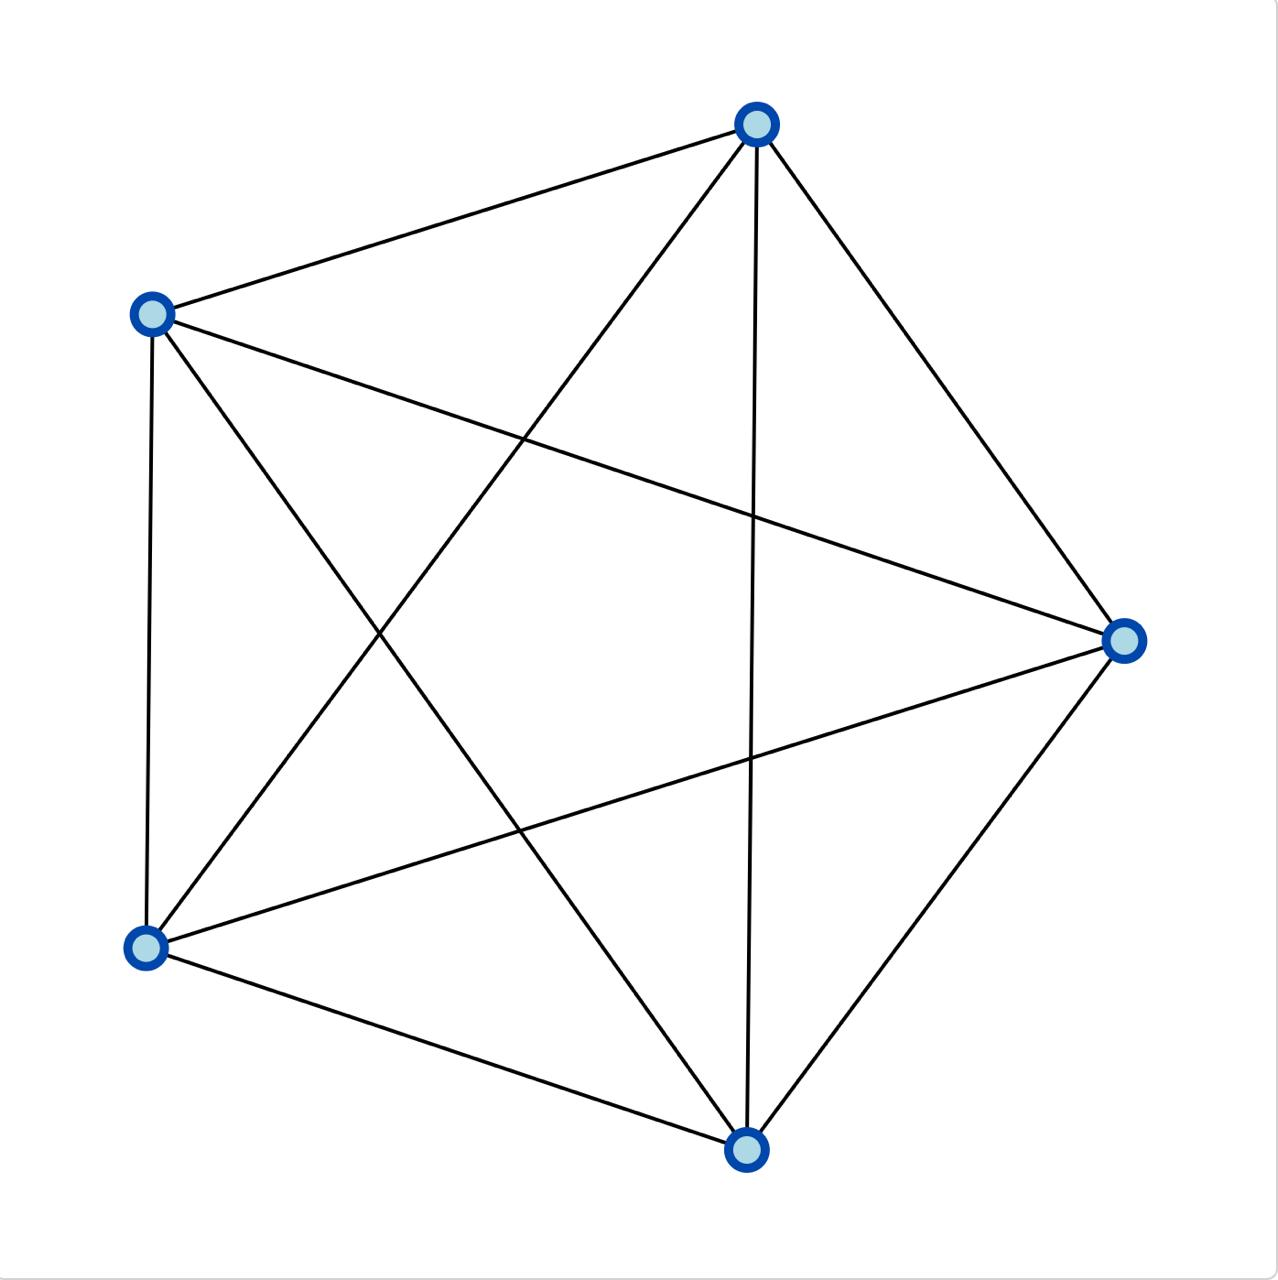
\includegraphics[width=0.5\textwidth]
{4.jpeg}  
    \caption{Граф $wg(G) = 4 , ir(G) = 5 $} 
    \label{fig:im2} 
\end{figure}


\begin{figure}[ht!]  
    \centering 
    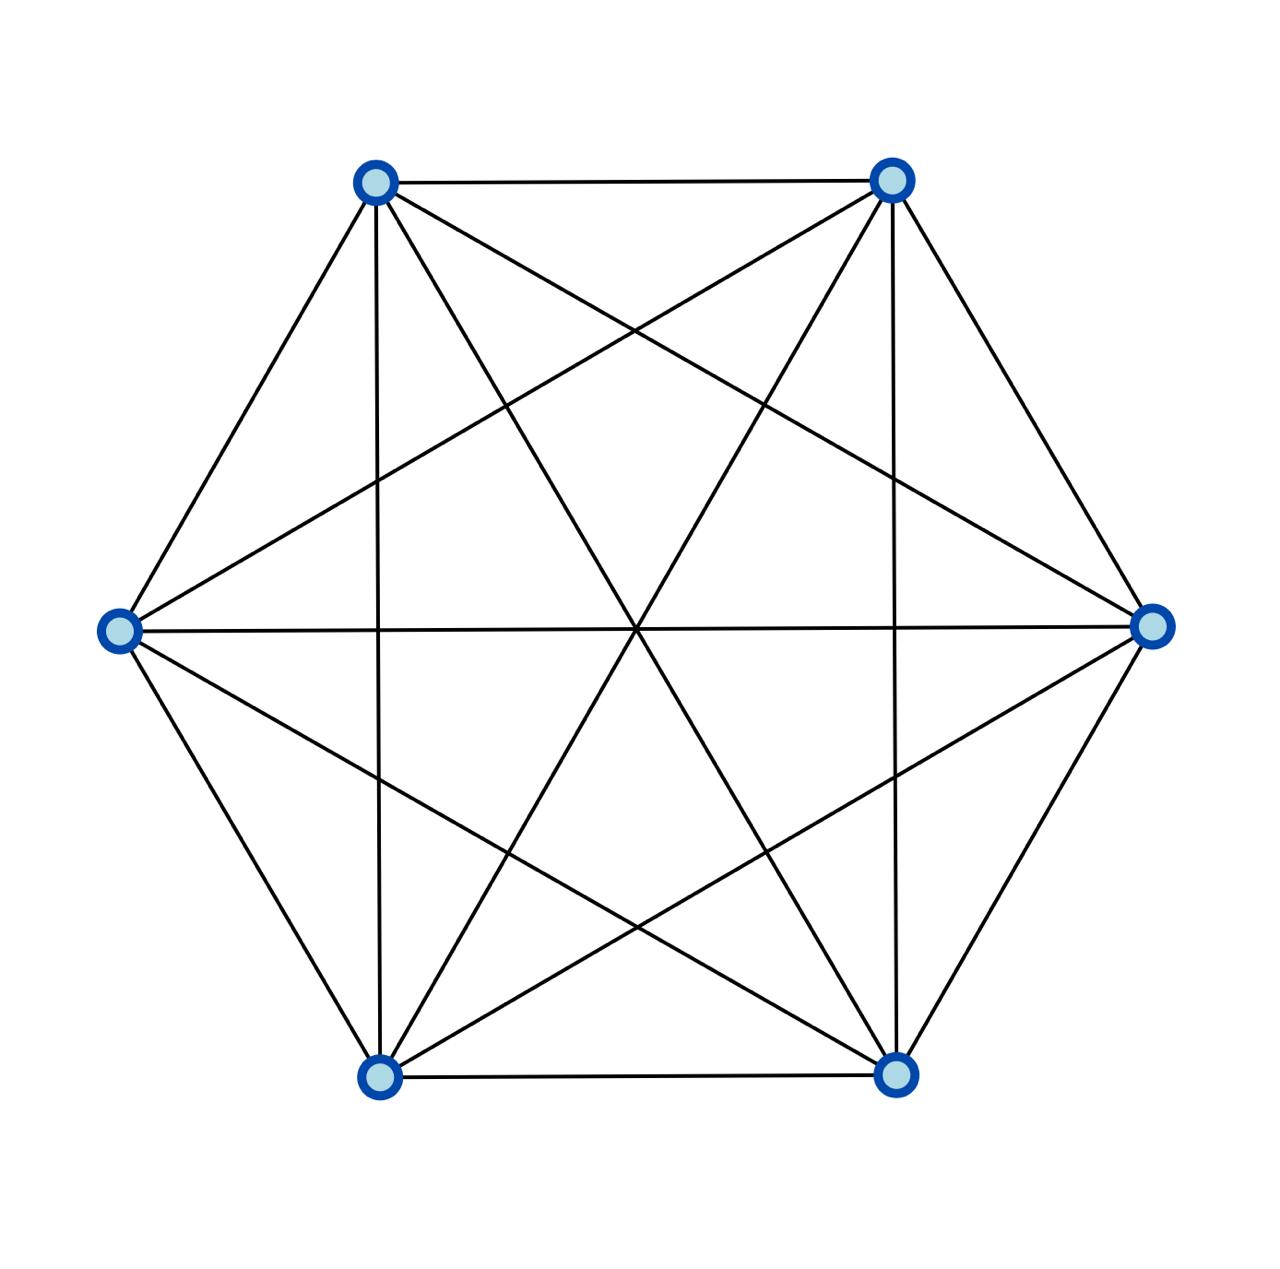
\includegraphics[width=0.5\textwidth]
{5.jpeg}  
    \caption{Граф $wg(G) = 5 , ir(G) = 6$} 
    \label{fig:im2} 
\end{figure}

\begin{figure}[ht!]  
    \centering 
    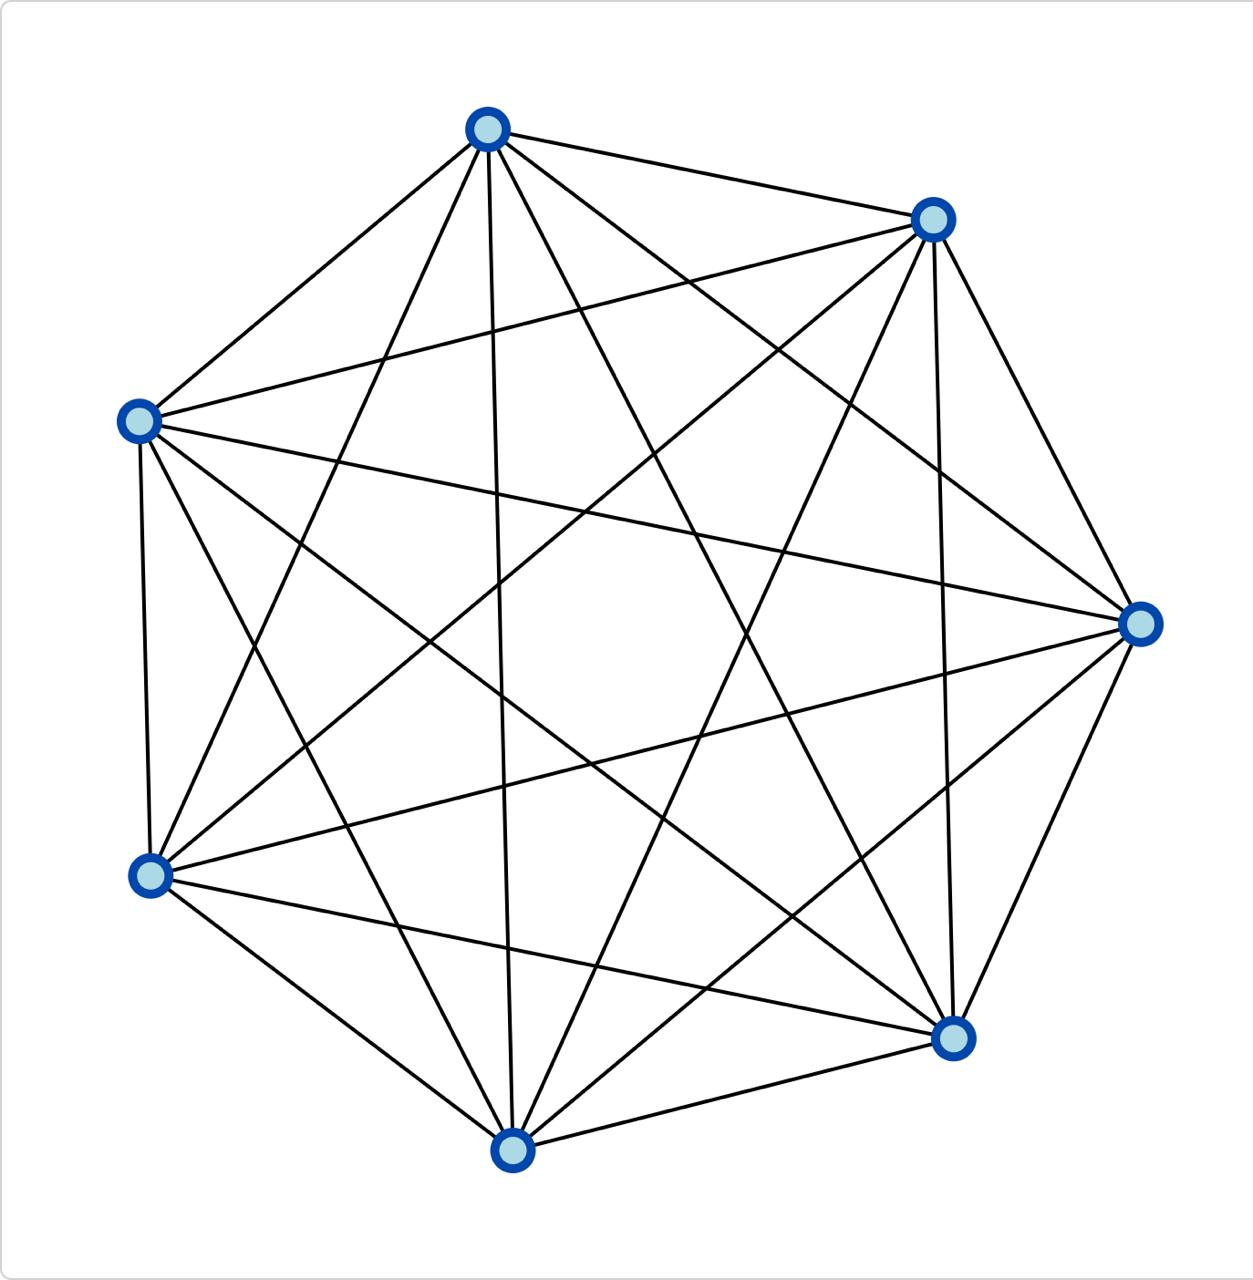
\includegraphics[width=0.5\textwidth]
{6.jpeg}  
    \caption{Граф $wg(G) = 6, ir(G) = 7$} 
    \label{fig:im2} 
\end{figure}

\begin{figure}[ht!]  
    \centering 
    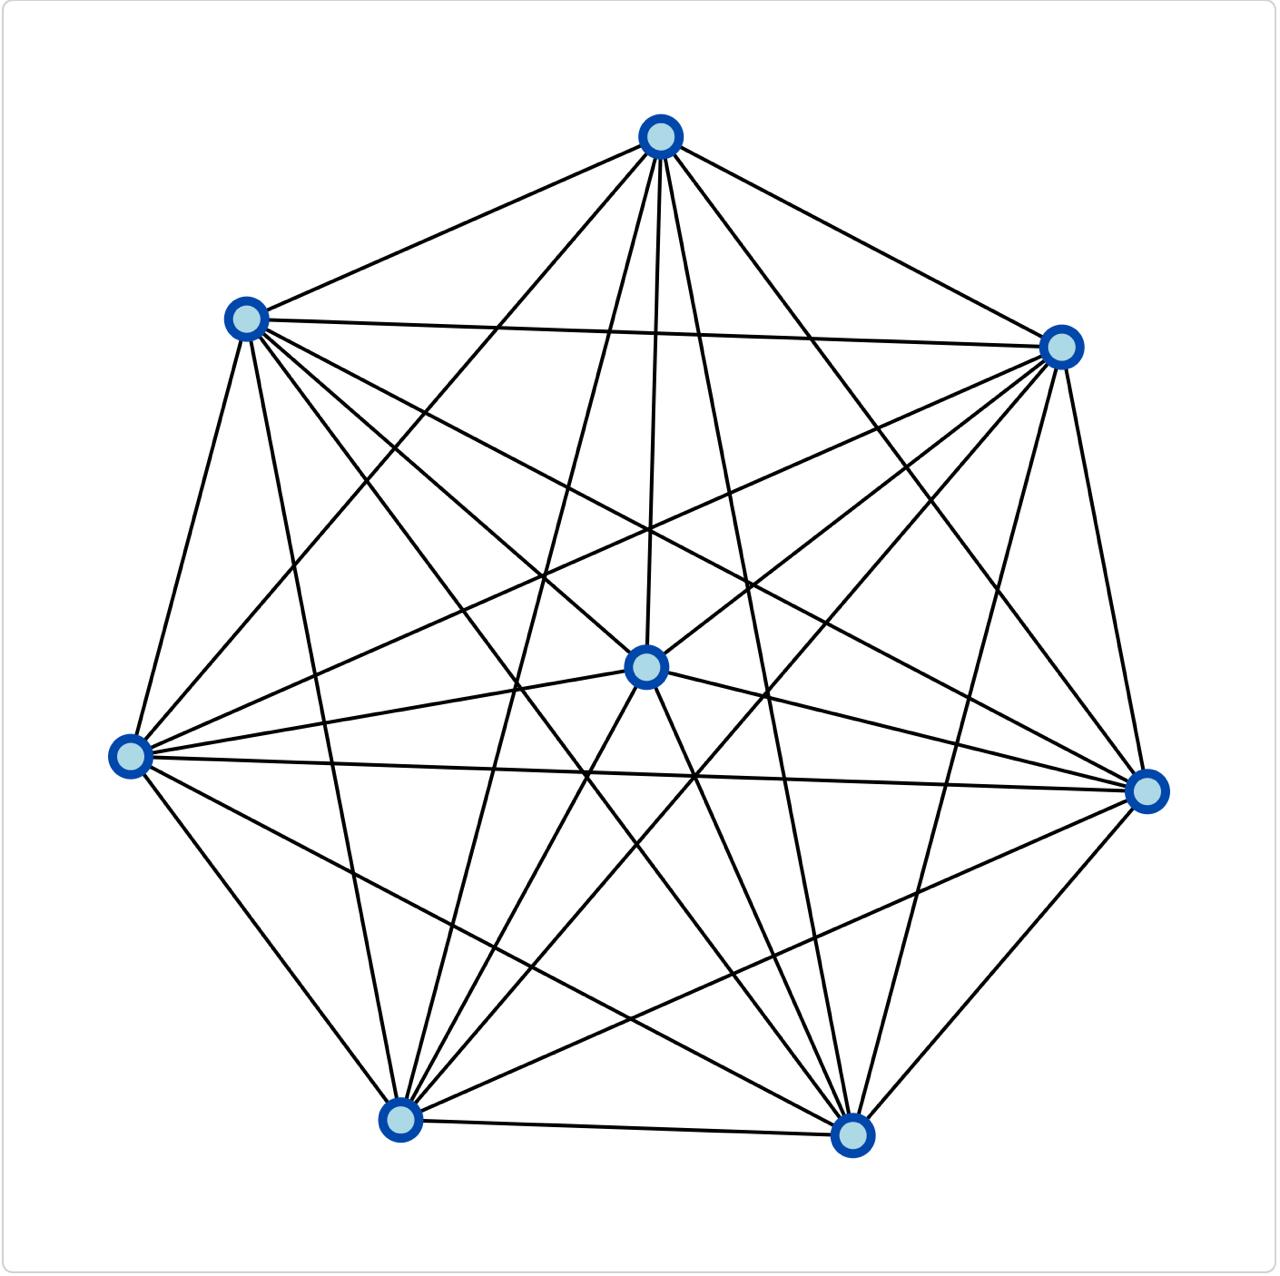
\includegraphics[width=0.5\textwidth]
{7.jpeg}  
    \caption{Граф $wg(G) = 7, ir(G) = 8$} 
    \label{fig:im2} 
\end{figure}

\begin{figure}[ht!]  
    \centering 
    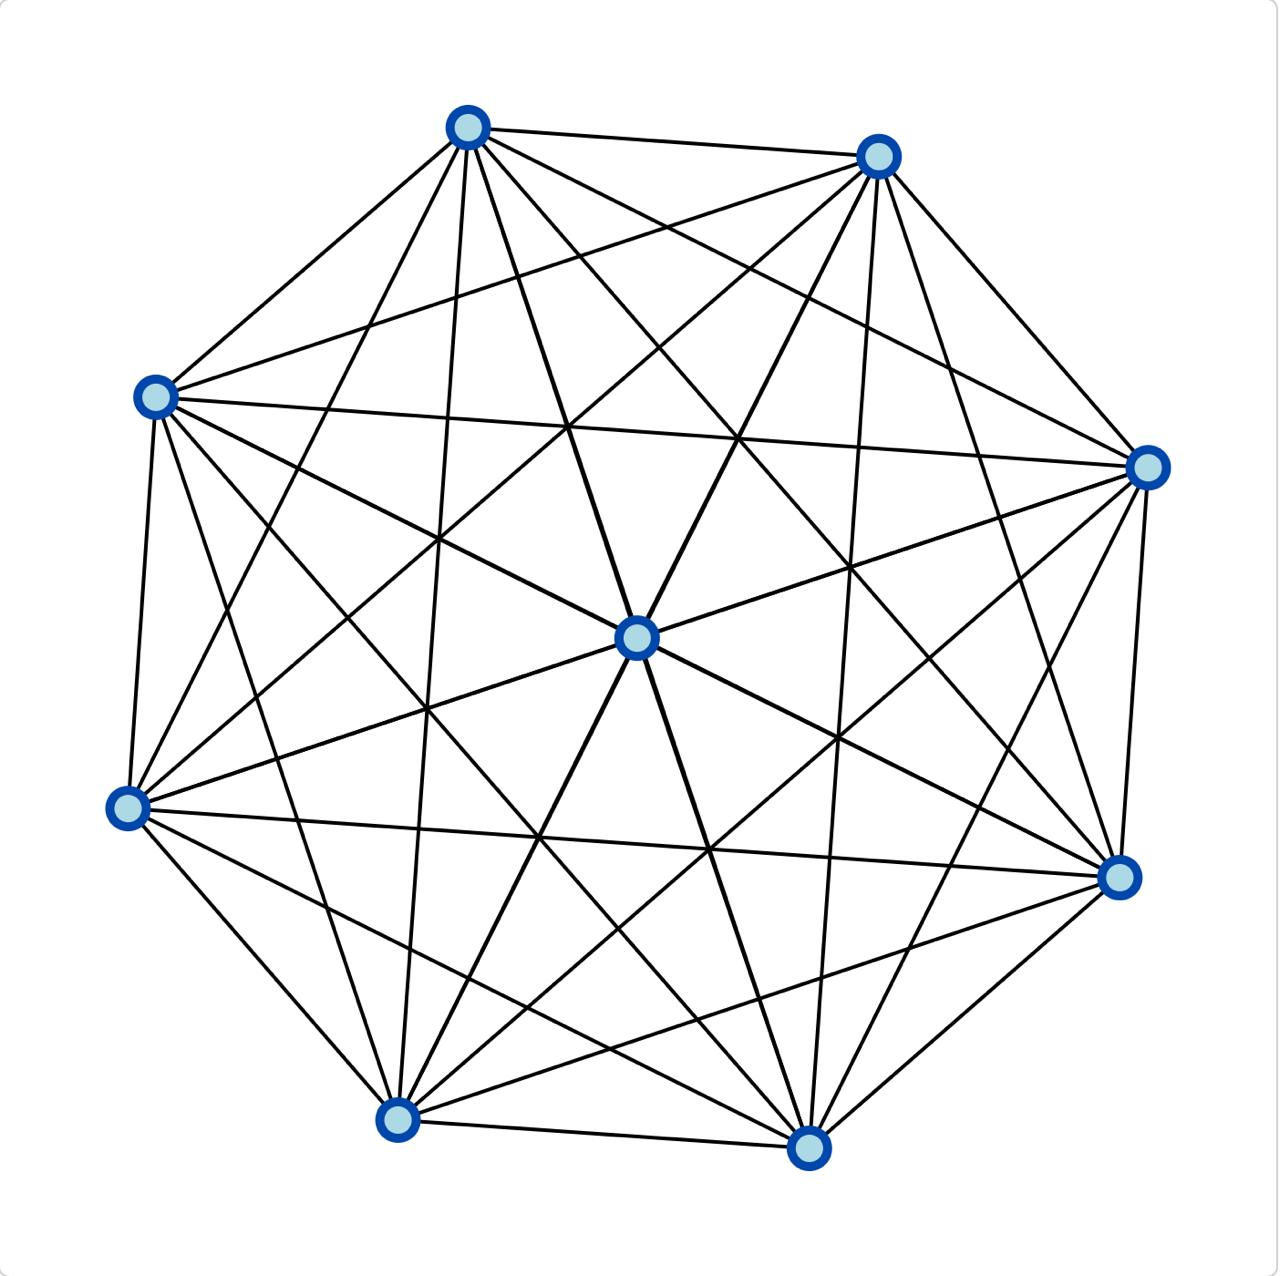
\includegraphics[width=0.5\textwidth]
{99.jpg}  
    \caption{Граф $wg(G) = 8, ir(G) = 9$} 
    \label{fig:im2} 
\end{figure}

\begin{figure}[ht!]  
    \centering 
    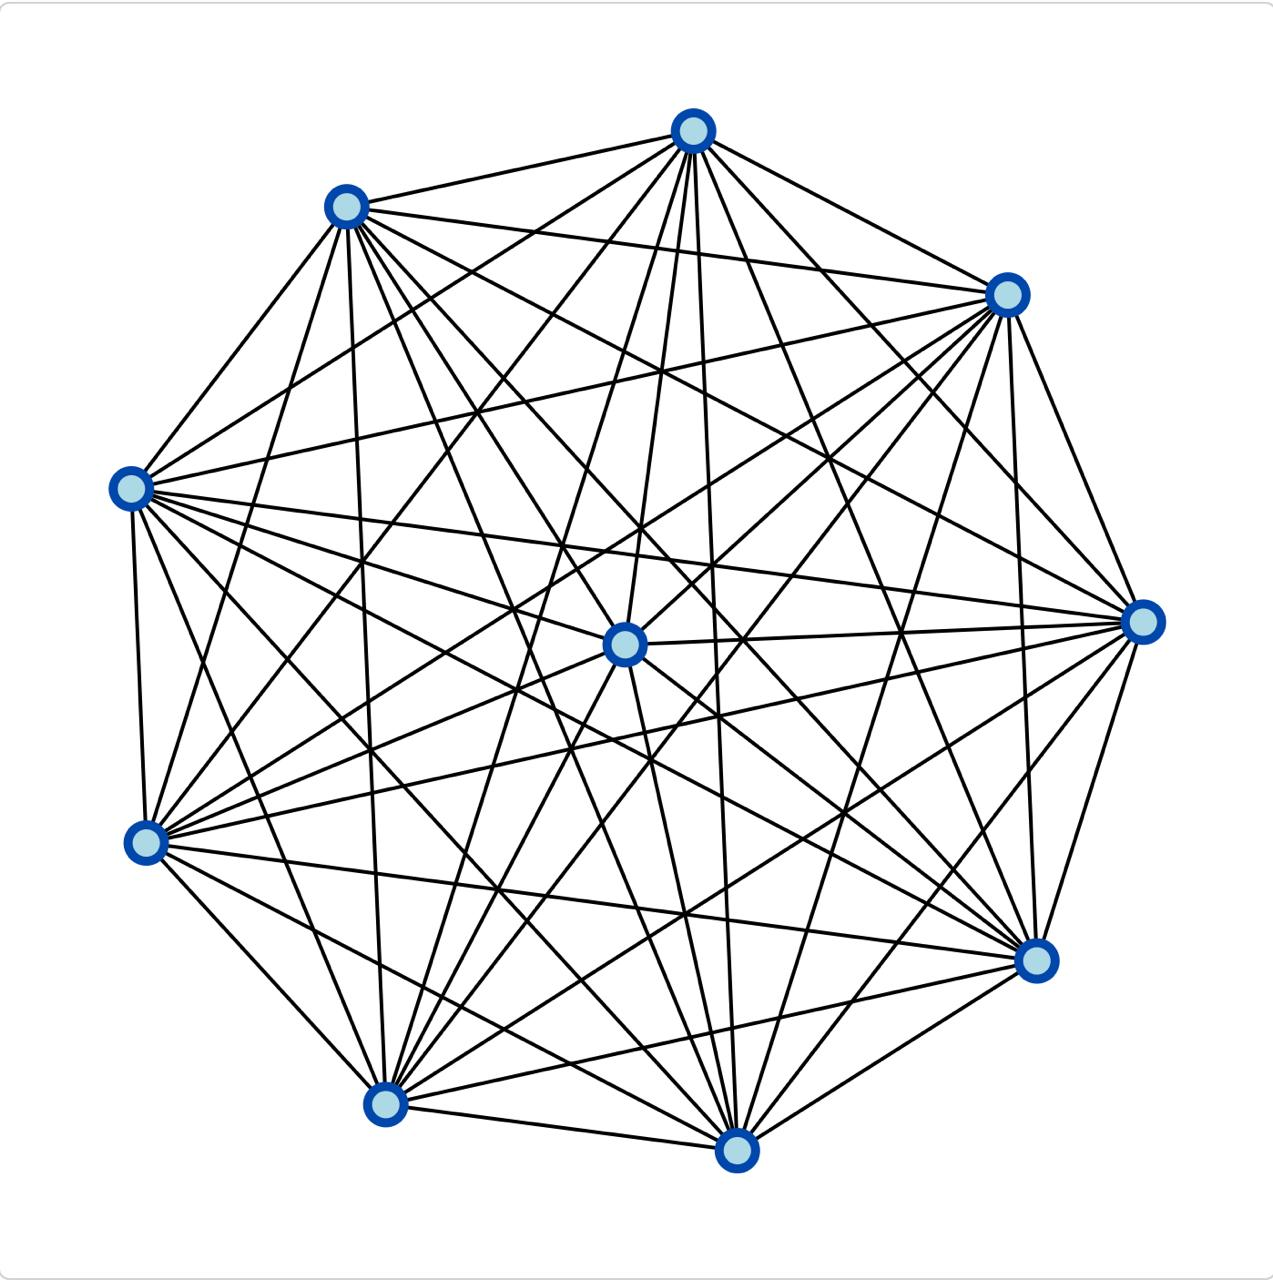
\includegraphics[width=0.5\textwidth]
{8.jpeg}  
    \caption{Граф $wg(G) = 9, ir(G) = 10$} 
    \label{fig:im2} 
\end{figure}


\begin{figure}[ht!]  
    \centering 
    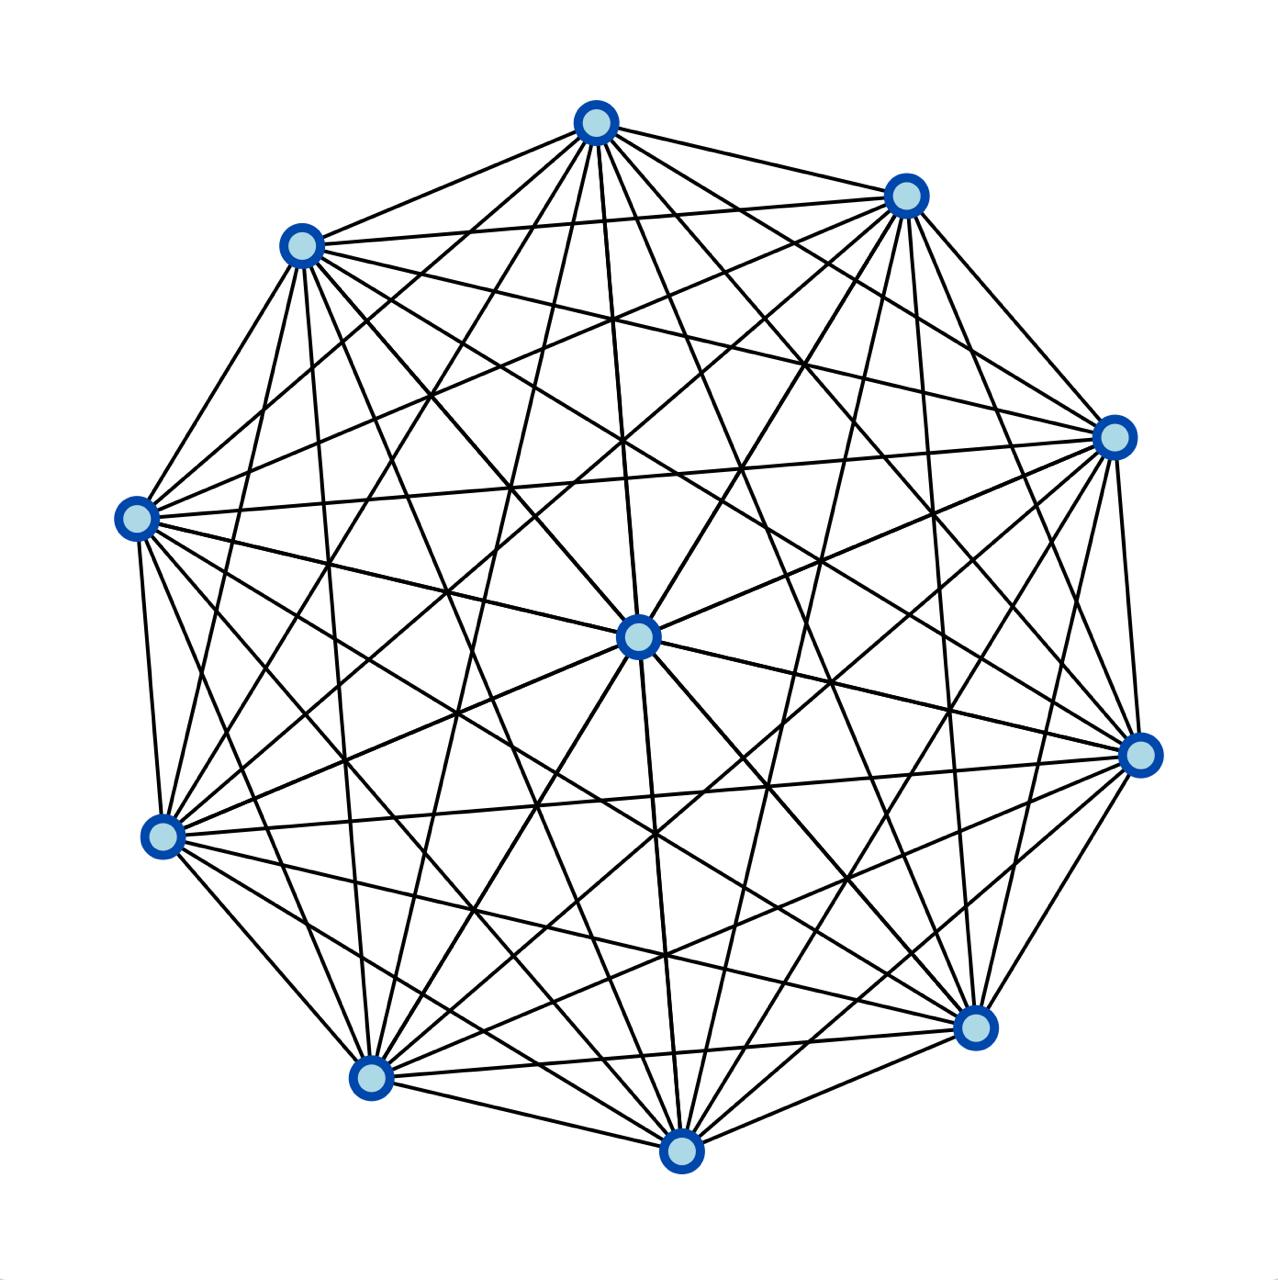
\includegraphics[width=0.5\textwidth]
{9.jpeg}  
    \caption{Граф $wg(G) = 10, ir(G) = 11$} 
    \label{fig:im2} 
\end{figure}
\newpage
На рисунках 20-26 представлены графы соответствующие гипотезе 2.

\begin{figure}[ht!]  
    \centering 
    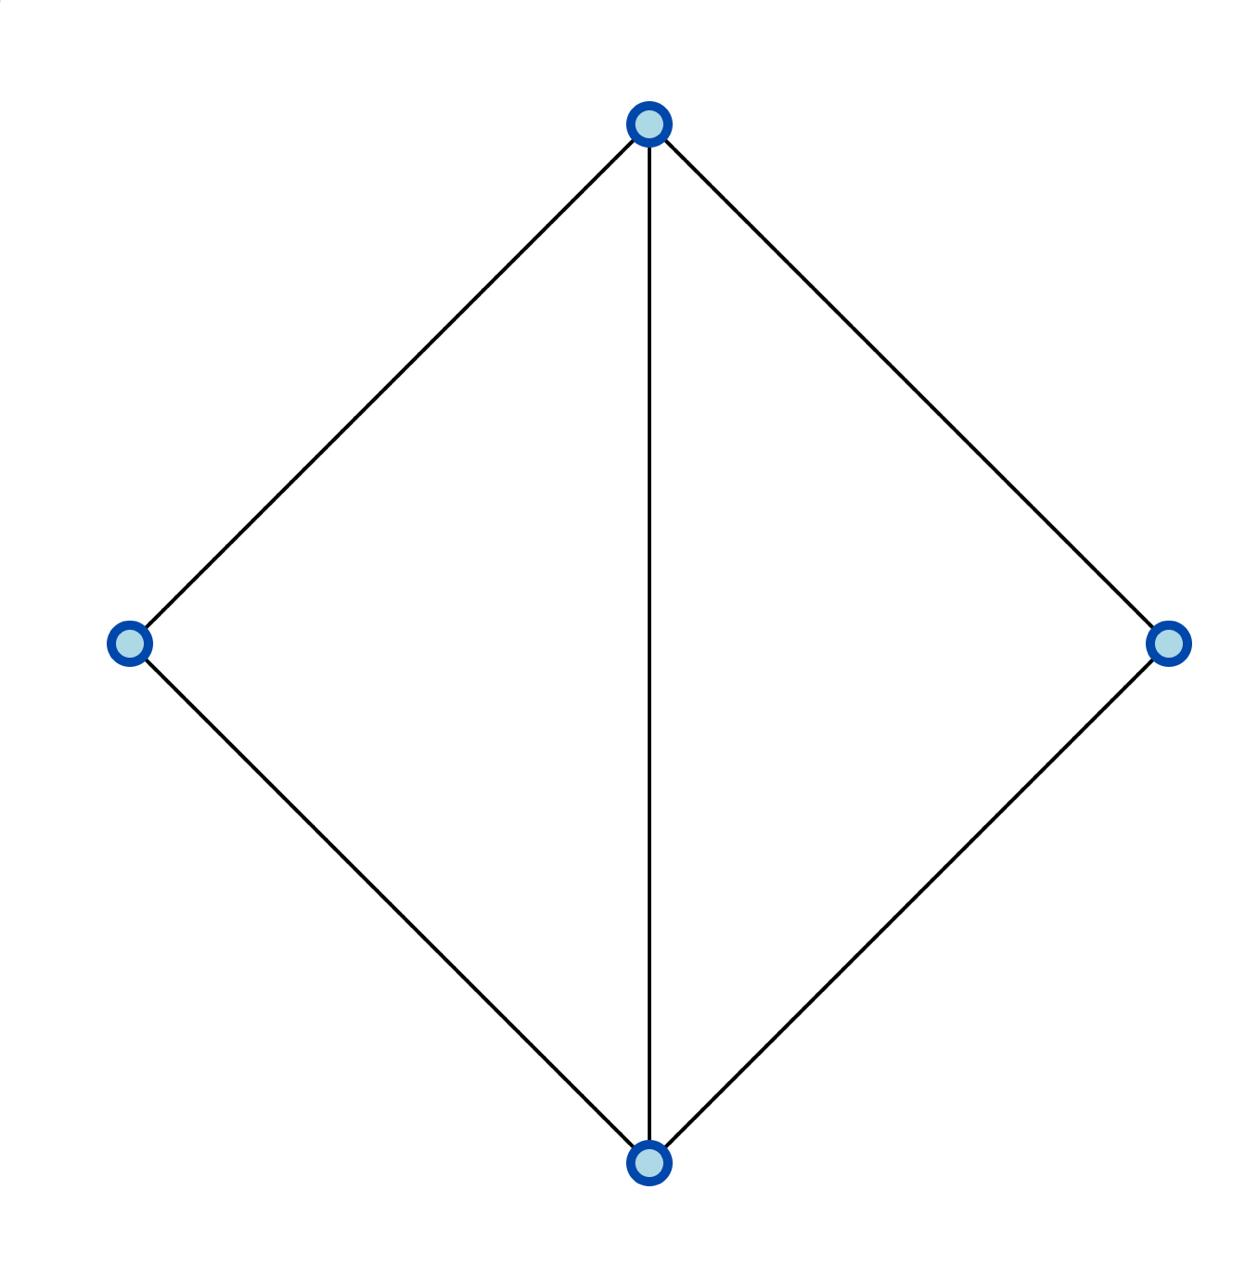
\includegraphics[width=0.5\textwidth]
{44.jpg}  
    \caption{Граф $wg(G) = ir(G) = 2$} 
    \label{fig:im3} 
\end{figure}

\begin{figure}[ht!]  
    \centering 
    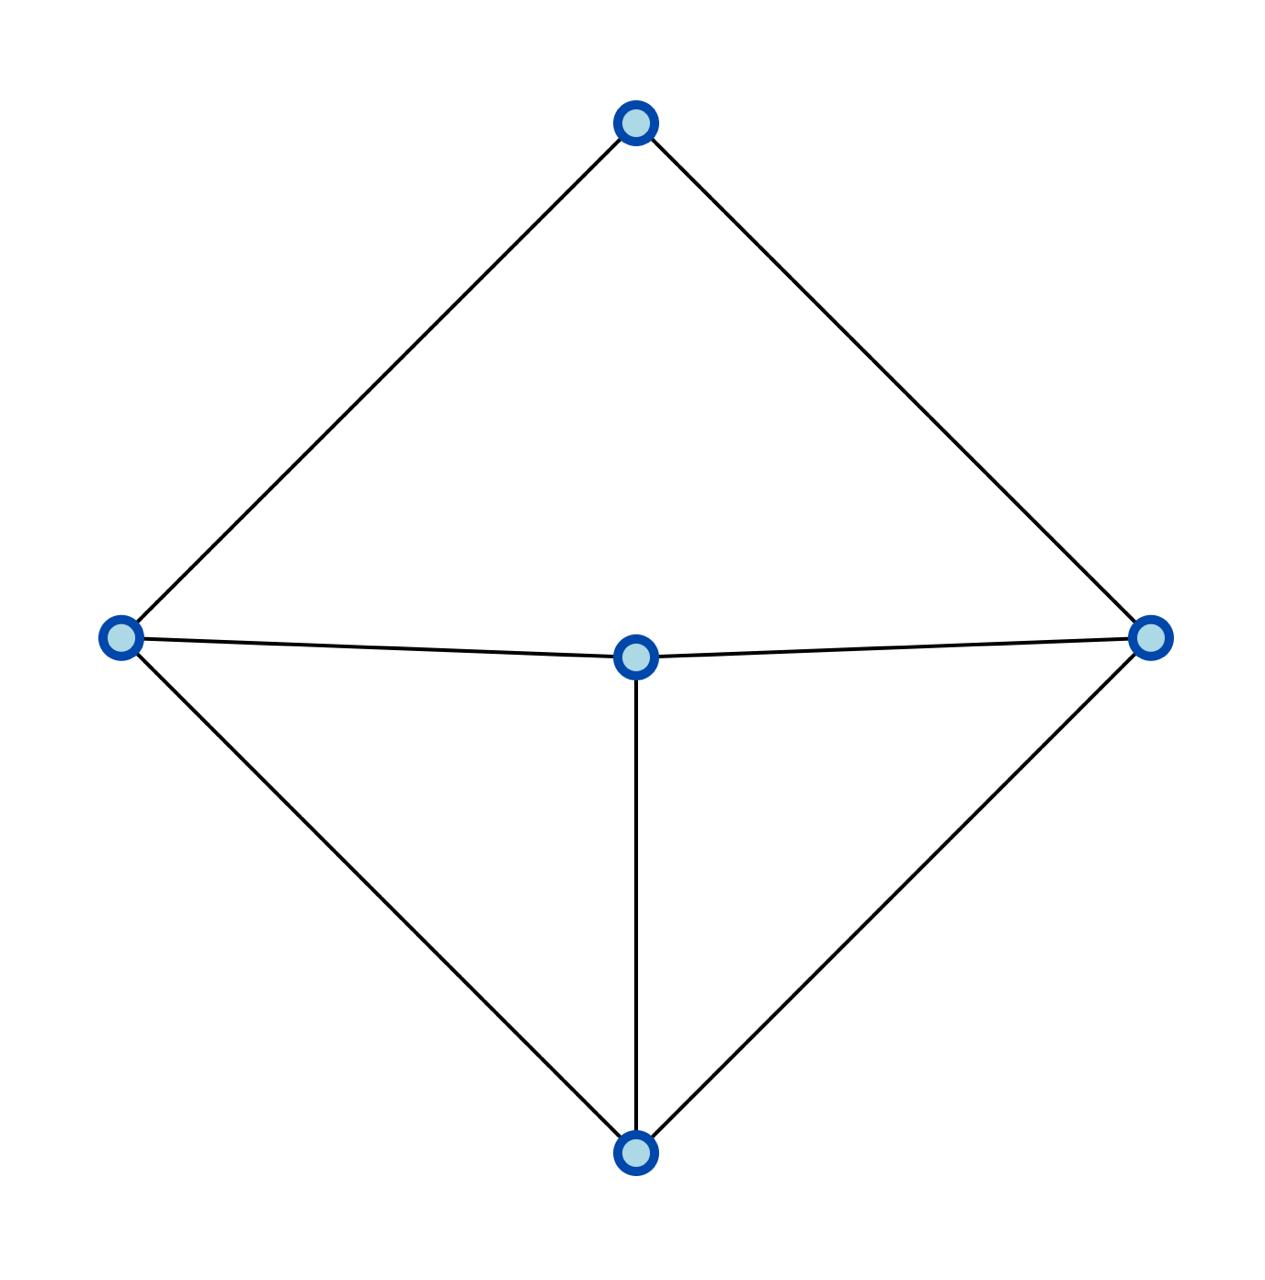
\includegraphics[width=0.5\textwidth]
{55.jpg}  
    \caption{Граф $wg(G) = ir(G) = 2$} 
    \label{fig:im3} 
\end{figure}

\begin{figure}[ht!]  
    \centering 
    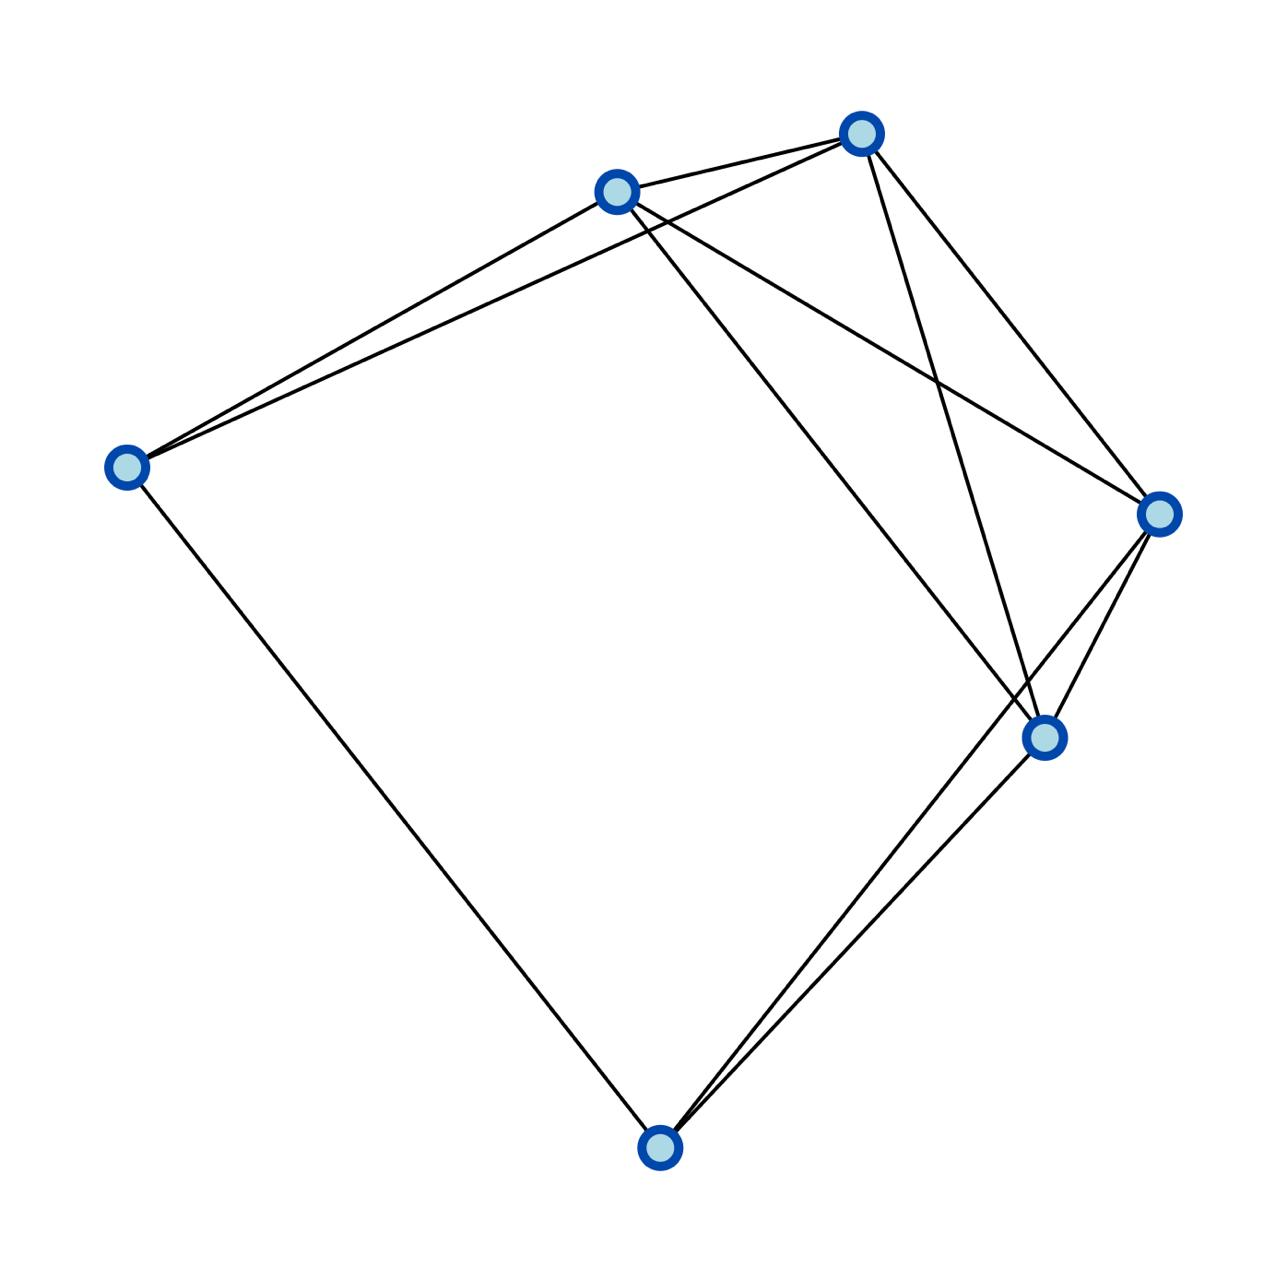
\includegraphics[width=0.5\textwidth]
{66.jpg}  
    \caption{Граф $wg(G) = ir(G) = 3$} 
    \label{fig:im3} 
\end{figure}

\begin{figure}[ht!]  
    \centering 
    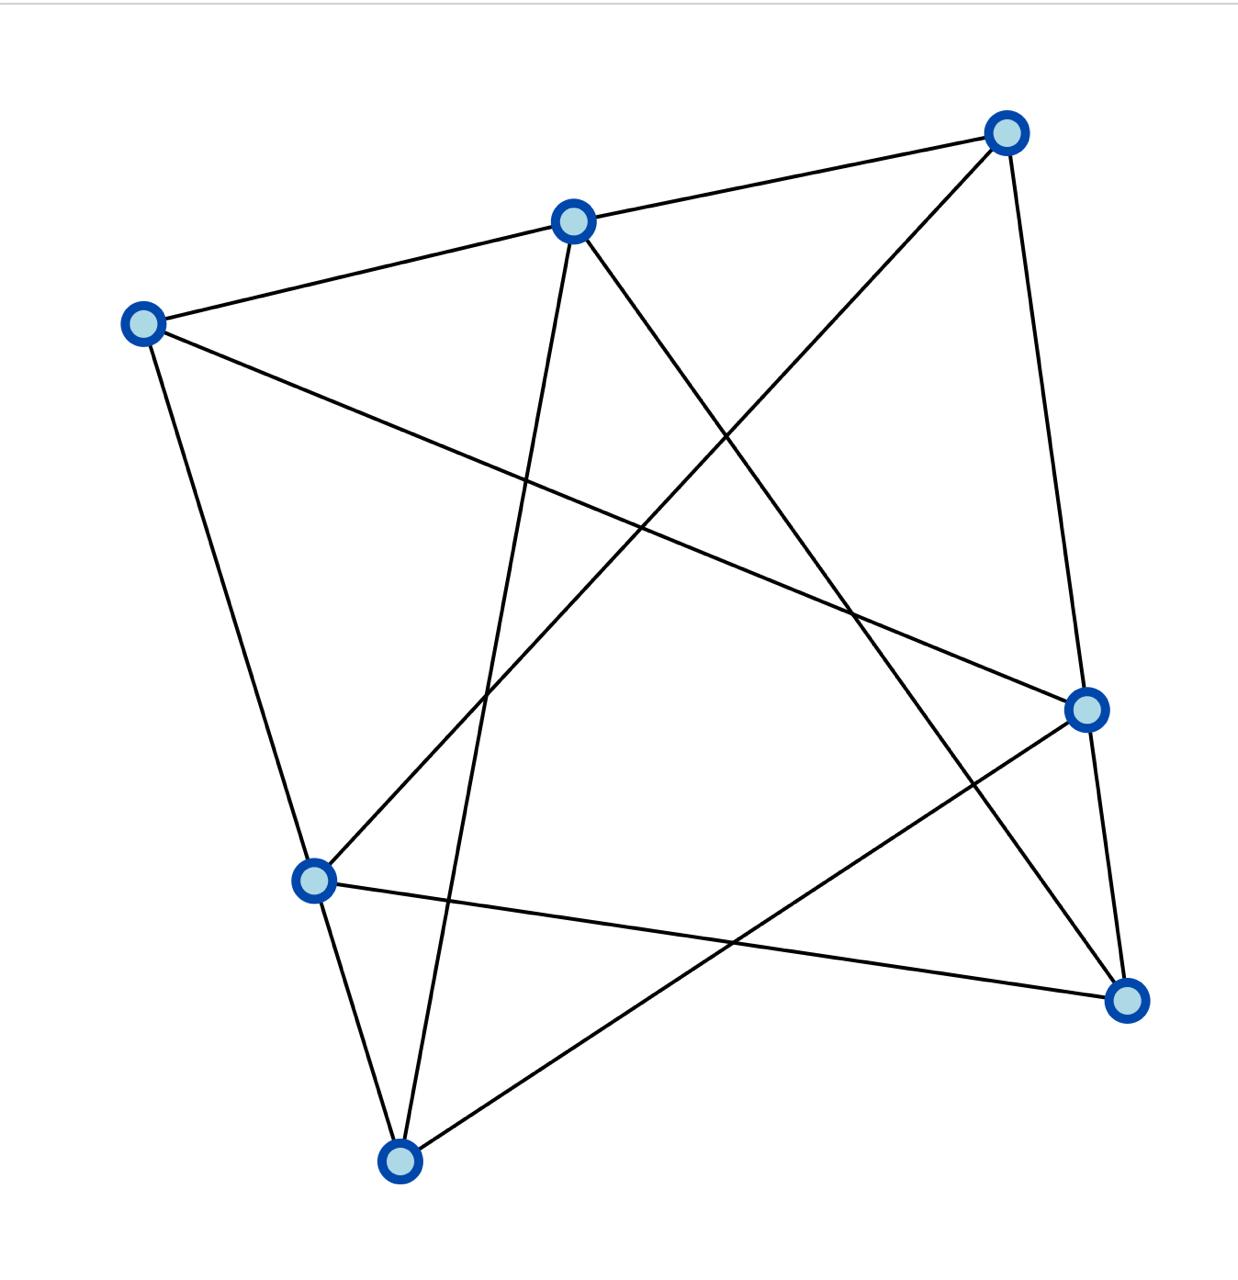
\includegraphics[width=0.5\textwidth]
{77.jpg}  
    \caption{Граф $wg(G) = ir(G) = 3$} 
    \label{fig:im3} 
\end{figure}

\begin{figure}[ht!]  
    \centering 
    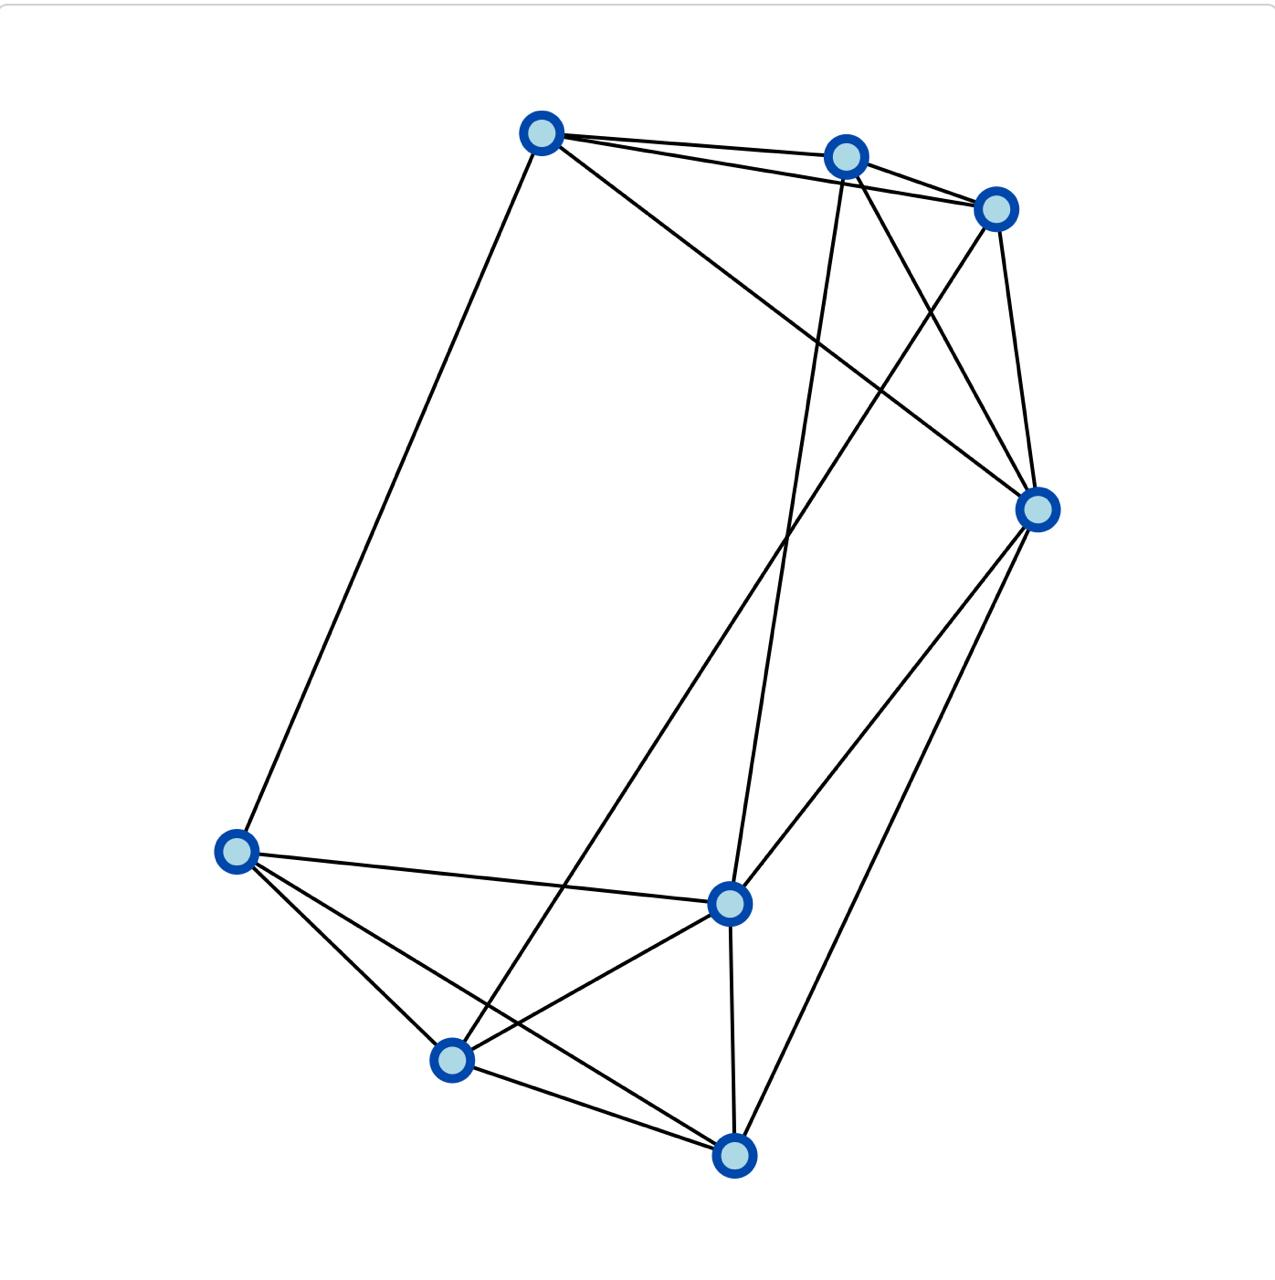
\includegraphics[width=0.5\textwidth]
{88.jpg}  
    \caption{Граф $wg(G) = ir(G) = 4$} 
    \label{fig:im3} 
\end{figure}

\begin{figure}[ht!]  
    \centering 
    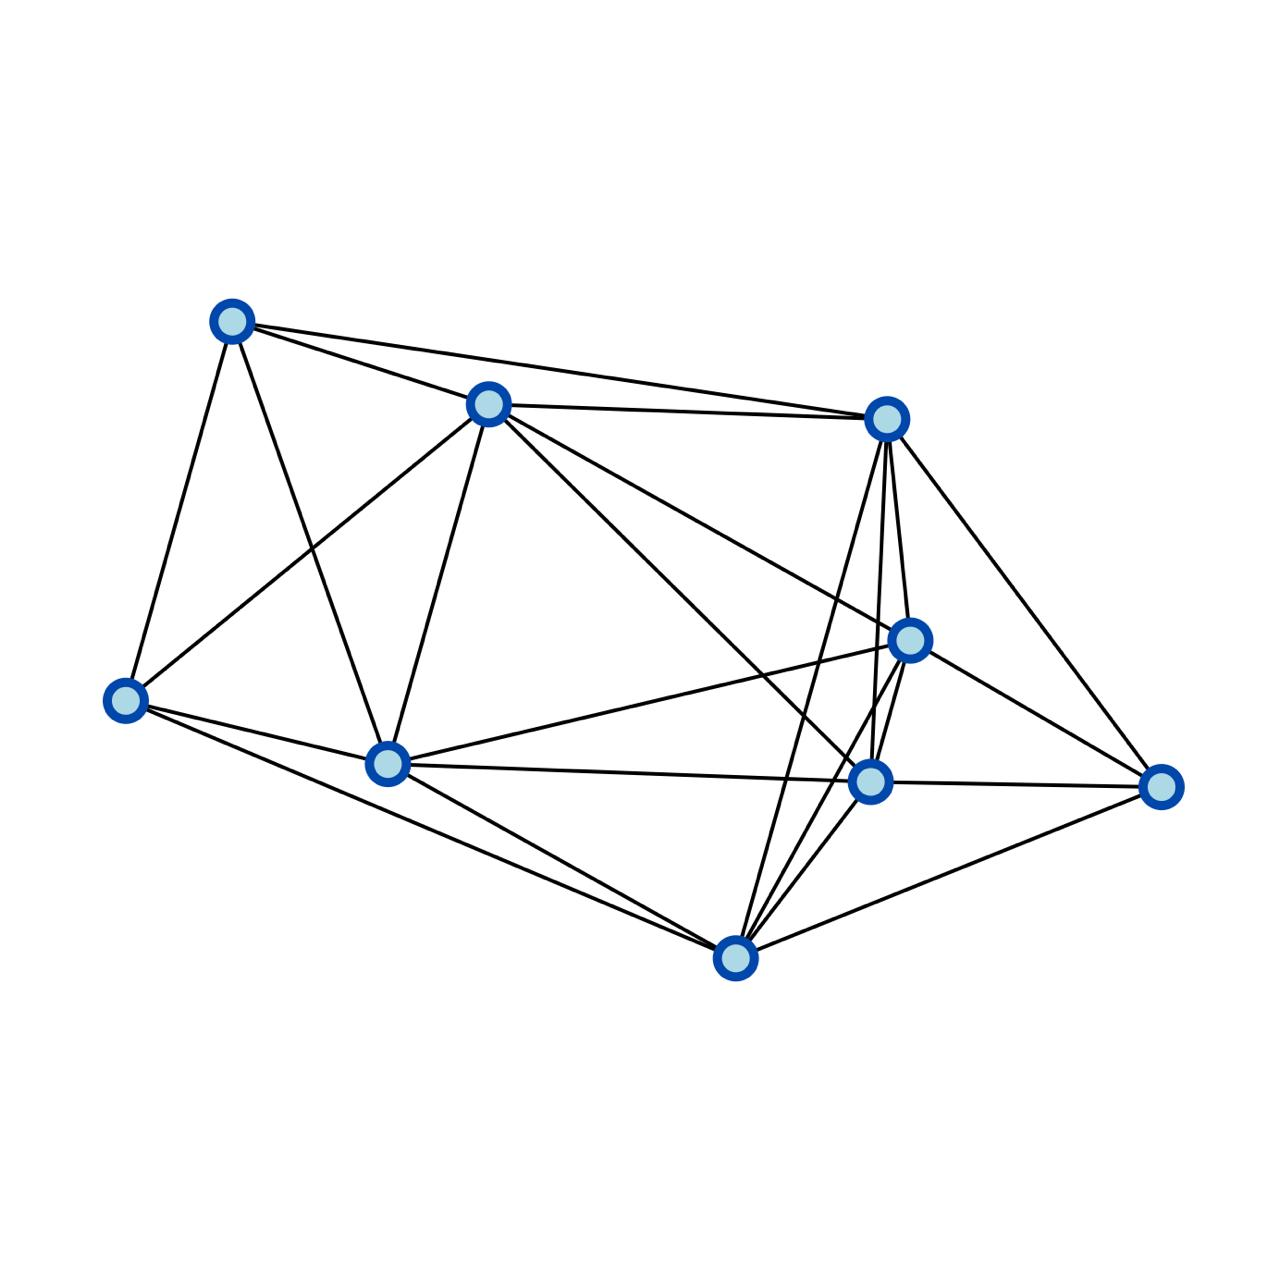
\includegraphics[width=0.5\textwidth]
{999.jpg}  
    \caption{Граф $wg(G) = ir(G) = 4$} 
    \label{fig:im3} 
\end{figure}
\FloatBarrier

\begin{figure}[h!]  
    \centering 
    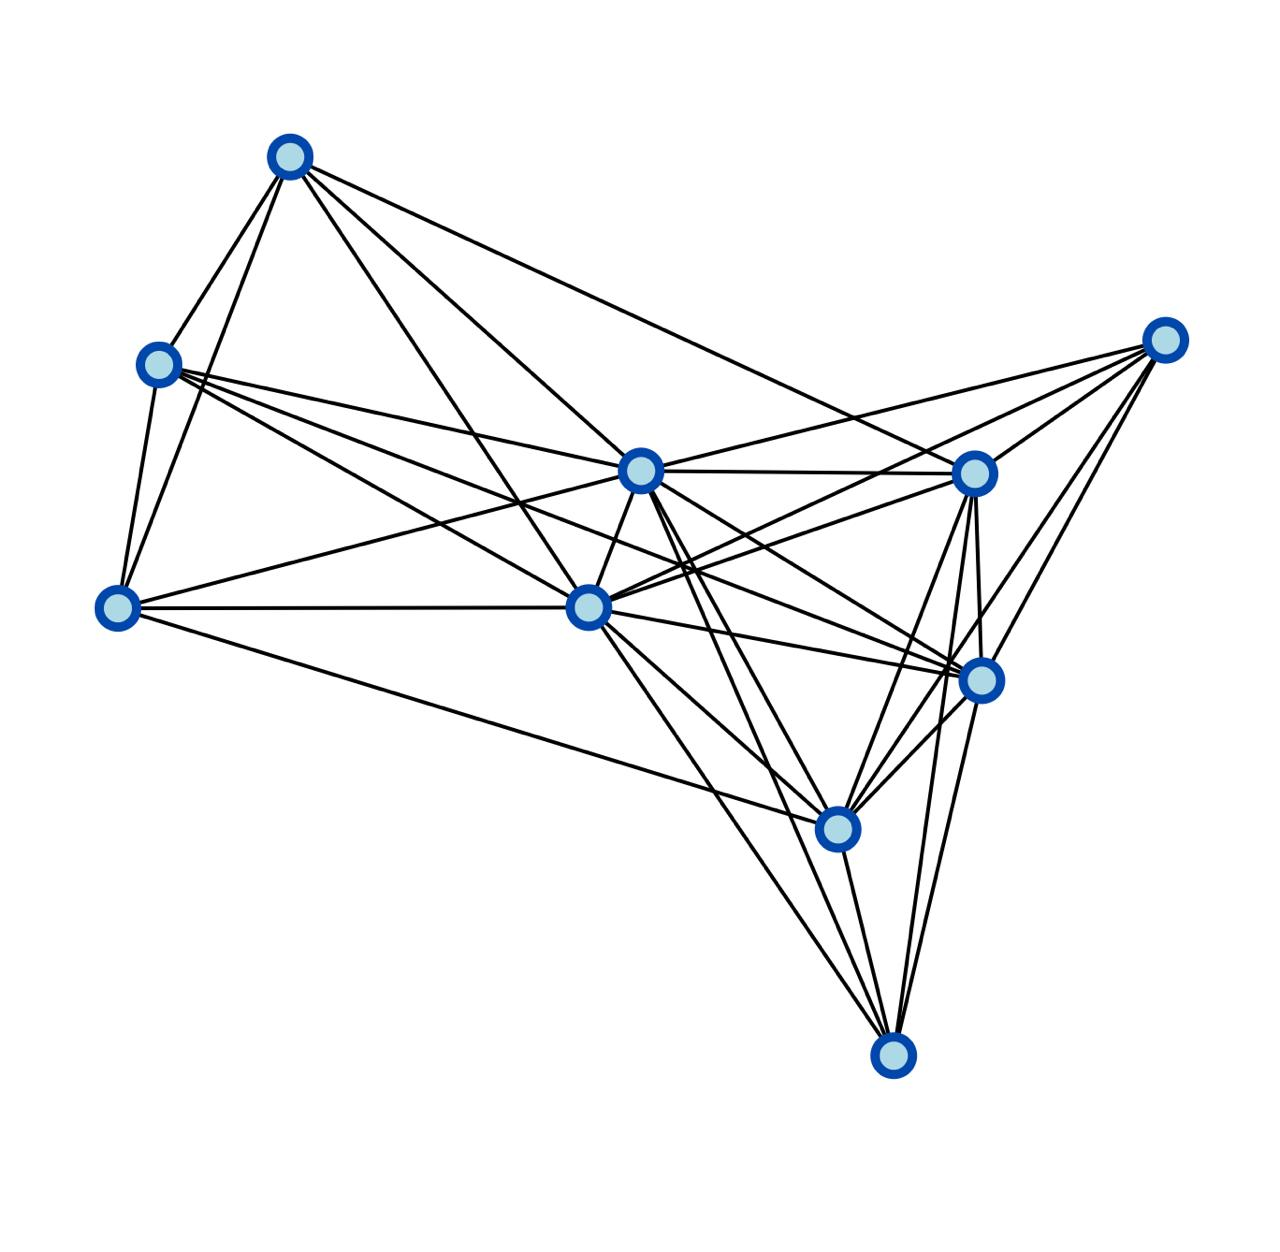
\includegraphics[width=0.5\textwidth]
{1010.jpg}  
    \caption{Граф $wg(G) = ir(G) = 5$} 
    \label{fig:im01} 
\end{figure}



\conclusion
В данной работе было проведено исследование инвариантов графов, в ходе которого был разработан алгоритм для нахождения слабого геодезического числа и числа несократимости графа. 
 В рамках вычислительных экспериментов изучены связные графы с количеством вершин до 11, что позволило получить важные статистические данные и выявить интересные закономерности в распределении рассматриваемых инвариантов.

Анализ полученных экспериментальных данных привел к формулированию следующих гипотез. В частности гипотеза о несуществовании графов с равными значениями инвариантов, начиная с определенного, об особенностях графов с максимальными значениями инвариантов, а также о количестве графов для минимального значения числа нескоратимости и максимального значения слабого геодезического числа.



\newpage
\bibliographystyle{ugost2003}
\bibliography{thesis}

\newpage
\appendix

\section{Листинг \texttt{main.py}}

\begin{minted}[]{python3}
import networkx as nx
import time
import itertools
from multiprocessing import Pool
import os
from collections import defaultdict
import itertools

def weak_geodetic_number(graph):
    nodes = list(graph.nodes())
    n = len(nodes)
    covered = set()
    S = set()
    
    shortest_paths_dict = defaultdict(dict)
    for u in nodes:
        for v in nodes:
            if u != v:
                try:
                    paths = list(nx.all_shortest_paths(graph, u, v))
                    shortest_paths_dict[u][v] = paths[0] if len(paths) == 1 else None
                except nx.NetworkXNoPath:
                    shortest_paths_dict[u][v] = None
            else:
                shortest_paths_dict[u][v] = [u]  

    all_pairs = list(itertools.combinations_with_replacement(nodes, 2))
    
    while len(covered) < n:
        best_gain = 0
        best_pair = None
        best_new_covered = set()
        
        for u, v in all_pairs:
            if u == v:
                new_covered = {u}
            else:
                path = shortest_paths_dict[u][v] or shortest_paths_dict[v][u]
                if path:
                    new_covered = set(path)
                    new_covered.add(u)
                    new_covered.add(v)
                else:
                    new_covered = {u, v}
            
            gain = len(new_covered - covered)
            if gain > best_gain:
                best_gain = gain
                best_pair = (u, v)
                best_new_covered = new_covered
                
                if len(covered | new_covered) == n:
                    break

        if best_pair is None:
            break
            
        S.update(best_pair)
        covered.update(best_new_covered)

    return len(S)

def is_irreducible(S, graph):
    if not S:
        return True 
    for v in S:
        pn = [u for u in S if u != v and not graph.has_edge(u, v)]
        if not pn:
            return False
    return True

def is_maximal_irreducible(S, all_nodes, graph):
    for w in all_nodes - S:
        extended = S | {w}
        if is_irreducible(extended, graph):
            return False
    return True


def connectivity_number(graph):
    V = set(graph.nodes)
    
    if not V:
        return 0

    min_size = float('inf')

    for r in range(len(V)+1):
        for subset in itertools.combinations(V, r):
            S = set(subset)
            if is_irreducible(S, graph) and is_maximal_irreducible(S, V, graph):
                min_size = min(min_size, len(S))

    return 1 if min_size == float('inf') else min_size



def process_single_graph(index, graph_string):
    """Обработка одного графа для параллелизации."""
    try:
        if not isinstance(graph_string, str):
            return {"index": index, "error": f"Неверный тип graph_string: {type(graph_string)}"}
        
        graph_string = graph_string.strip()
        if not graph_string:
            return {"index": index, "error": "Пустая строка Graph6"}
        
        graph = nx.from_graph6_bytes(graph_string.encode())
        
        start_time = time.time()
        wg_number = weak_geodetic_number(graph)
        wg_time = time.time() - start_time
        connectivity = connectivity_number(graph)
        conn_time = time.time() - start_time

        return {
            "index": index,
            "graph": graph_string,
            "weak_geodetic_number": wg_number,
            "weak_geodetic_time": wg_time,
            "connectivity_number": connectivity,
            "connectivity_time": conn_time
        }
    except Exception as e:
        return {"index": index, "error": f"Ошибка обработки графа: {str(e)}"}


def process_single_graph_star(args):
    return process_single_graph(*args)

def process_graph6_file(file_path):
    """Обработка файла Graph6 с оптимизированной параллелизацией"""
    results = []
    start_time_total = time.time()
    
    if not os.path.exists(file_path):
        print(f"Ошибка: Файл {file_path} не существует")
        return results, 0
    
    try:
        with open(file_path, 'r') as file:
            graph_strings = [line.strip() for line in file if line.strip()]
    except Exception as e:
        print(f"Ошибка чтения файла {file_path}: {str(e)}")
        return results, 0
    
    if not graph_strings:
        print(f"Ошибка: Файл {file_path} пуст или содержит только пустые строки")
        return results, 0
    

    num_processes = min(os.cpu_count() or 8, 10, len(graph_strings))
    print(f"Используется {num_processes} процессов")
    

    chunk_size = max(1, len(graph_strings) // (num_processes * 4))
    
    try:
        with Pool(processes=num_processes) as pool:

            results = list(pool.imap_unordered(
                process_single_graph_star,
                enumerate(graph_strings),
                chunksize=chunk_size
            ))
    except Exception as e:
        print(f"Ошибка при параллельной обработке: {str(e)}")
        return results, time.time() - start_time_total
    
    total_time = time.time() - start_time_total
    return results, total_time

def main():
    start_time_global = time.time()
    total_graphs = 0
    total_errors = 0
    result = [[0 for _ in range(11)] for _ in range(11)]
    with open(input_file, 'r') as f:
        for i in range(0, 10):
            for j in range(0, 10):
                input_file = f"./graph/outt10_00{i}{j}"
                input_file = f"./graph/res7.txt"
                print(f"\nОбработка файла: {input_file}")
                results, total_time = process_graph6_file(input_file)
                time_total1 = 0
                time_total2 = 0
                real_w_g = {}
                real_c_n = {}
                count = 0
                errors = 0
                
                for result in results:
                    if "error" in result:
                        errors += 1
                        total_errors += 1
                        continue
                        
                    count += 1
                    time_total1 += result['weak_geodetic_time']
                    time_total2 += result['connectivity_time']
                    
                    w_g = result['weak_geodetic_number']
                    c_n = result['connectivity_number']
                    
                    real_w_g[w_g] = real_w_g.get(w_g, 0) + 1
                    real_c_n[c_n] = real_c_n.get(c_n, 0) + 1
                    if w_g < 11 and c_n < 11:
                        result[w_g][c_n] += 1
                total_graphs += count

                print("\nМатрица [wg][connectivity]:")
                print("     " + " ".join([f"{i:>4}" for i in range(11)]))
                for i in range(11):
                    row = " ".join([f"{result[i][j]:>4}" for j in range(11)])
                    print(f"{i:>3}: {row}")
                
                f.write(f"Номер итерации {i}{j}")
                f.write(f"Всего графов: {count}")
                f.write(f"Ошибок: {errors}")
                f.write(f"Суммарное время слабого геодезического числа: {time_total1:.4f} сек")
                f.write(f"Распределение по значению инварианта:")
                f.write(f"1. Слабое геодезическое число: {real_w_g}")
                f.write(f"Общее время обработки файла: {total_time:.4f} сек")
               
                total_time_global = time.time() - start_time_global
                print("\nИтоговая статистика:")
                print(f"Всего обработано графов: {total_graphs}")
                print(f"Общее количество ошибок: {total_errors}")
                print(f"Общее время выполнения: {total_time_global:.4f} сек")

if __name__ == "__main__":
    main()

\end{minted}

\end{document}

